\documentclass{article}
\usepackage[margin=1.5in]{geometry}
\usepackage[utf8]{inputenc}
\usepackage{mathrsfs,amsmath} 
\usepackage{amssymb}

\usepackage{algorithm}
\usepackage{algpseudocode}

\usepackage{caption}
\usepackage{subcaption}
\usepackage{url}
\usepackage{graphicx}
\usepackage{subfig}
\usepackage{graphicx}
\DeclareMathOperator*{\argmax}{arg\,max}
\graphicspath{ {./images/} }
\title{Deep Multi-Agent Reinforcement Learning in Starcraft II}
\author{Nicholas Burden}
\date{Trinity 2020}

\begin{document}

\maketitle
\thispagestyle{empty}
\vfill
\vfill
\begin{center}
    
\includegraphics[scale=0.2]{images/ox_logo.png}
\end{center}

\newpage


\begin{abstract}
    Deep Multi-Agent Reinforcement Learning (DMARL) is a rapidly advancing subfield within AI owing to its ability to learn end-to-end control policies from high-dimensional input states, allowing the acquisition of super-human game play skills across a variety of domains. One particularly prominent benchmark suite in the space of partially observable multi-agent games is the Starcraft Multi-Agent Challenge (SMAC) \cite{smac}, which is based on challenging StarCraft II unit micromanagement tasks. 
While SMAC tasks are diverse, they do draw from a small finite set of unit types and give rise to locally similar observations. We therefore hypothesise that it should be possible to both train policies that can generalise over previously unseen tasks, as well to warm-start training of difficult large-scale tasks using policy weights from similar small-scale tasks.
However, the state-of-the-art multi-agent learning algorithm QMIX \cite{qmixcite} has a network architecture that may admit a different number of weights for tasks with different numbers of agents and enemies.  
In order to construct a universal network architecture for QMIX's utility functions, we first equip it with grid input representations and then perform a comprehensive investigation of the relative performance of a variety of convolutional network architectures. We find that combining grid-based input representations with an additive mixing function (VDN \cite{vdn}) helps construct a universal multi-agent architecture that better generalises over scenarios with different numbers of agents and enemies and that, surprisingly, good training performance can be reached with much less input information than previously assumed.
\end{abstract}
\newpage
\tableofcontents
\newpage
\section{Introduction}
Reinforcement Learning (RL) is an extremely relevant and successful approach to many modern problems. In recent years, great proficiency in complex tasks such as Go \cite{go} and Resource Management \cite{resourcemanagement} has been achieved using RL. These successes are important as the RL algorithms employed are general, and can easily be applied to other domains, while more traditional approaches to AI are specific to the problem at hand. 

Multi-agent RL is a natural next step, where multiple agents must co-operate to achieve a common goal. Some success has already been made in this space, examples being a multi-agent approach to traffic light co-ordination systems \cite{traffic} and (more specific to the domain of this project) superhuman proficiency in Starcraft II \cite{alphastar}, a popular real-time strategy video game. These advances are incredibly relevant to AI, as the world is inherently multi-agent: almost every AI problem can be viewed as a co-operation task between various actors. Success in this domain is integral to the advancement of AI and machine learning as a whole.

This project focuses on the role of multi-agent RL in Starcraft II video game in the form of a general RL algorithm for multiple co-operating agents. A key part of this project will be working towards an approach that is independent of the number of units in the map, a feature that is not seen in \cite{alphastar}. This is important as it makes the RL algorithm more general, and allows for transfer learning to different scenarios. This will involve a new approach to a state and action abstraction, as well as comprehensive experiments to determine the viability of these approaches, and compare their performance to standard approaches.

\subsection{The Challenge of Starcraft}

Starcraft II is a real-time strategy video game made by Blizzard Entertainment. It is a challenging game that has been played in esports tornaments for over 20 years.

Games are generally played with one player against another, each choosing to play as an alien race: Zerg, Protoss or Terran, with each having different charcacteristics. The game involves using workers to gather resources, which can make more units and buildings, as well as using other units to attack the enemy player. In this way, a successful player is able to manage the long-term overall structure of their team, know as macromanagement, as well as manage the lower level actions of individual units, know as micromanagement. This project will focus on micromanagement, as this is generally seen as a limiting factor for the competency of a player.

The game is challenging for a number of reasons. Firstly, as with game theory, the state of the game is constantly altered by both players, so there is no ``best strategy''. This style of game requires constant adaptation to the opponent's move, and must be responsive in this way to succeed. 

Furthermore, each agent suffers from a lack of information. In the implementation of the environment we will use, each agent has a limited field of view, so must make use of what it can, and has historically, observed. To overcome this problem, this project will explore the use of recurrent neural networks, which allow for past data to be used to make a present decision.

Starcraft is a difficult application of reinforcement learning as the action space can be extremely large. As well as moving to any place on the map, the unit is able to attack any enemy unit within its field of view, and can also perform special moves, such as healing. Approaches to overcome this problem must be made, such as restricting movement to one of four directions at a time, in order to reduce the size of this action space. 

Finally, as mentioned before, a significant part of this project will be working towards an architecture that is independent of the number of units in the game. The action space is dependent on this, since for each enemy unit, the agent has an attack action. Other observations, such as the agent's identifier, are also dependent on the number of agents (each identifier is represented as a binary string), which is also undesirable as it reduces generality. A key goal of this project is to allow for transfer learning over different scenarios, for which we must rid of this dependency.

\subsection{Recent Work}

Due to its difficulty, Starcraft II is an attractive domain for Machine Learning (ML). AlphaStar has demonstrated success in this domain \cite{alphastar}, recently beating one of the top professional players, Team Liquid’s Grzegorz ``MaNa'' Komincz, 5-0. AlphaStar uses deep neural networks for multi-agent reinforcement learning, training using data from both human and data games \cite{alphastar}. AlphaStar uses neural network to represent a central policy, which is also conditioned over a statistic $z$ that summarizes a strategy sampled from human data \cite{alphastar}. Overall, AlphaStar has achieved grandmaster status in all three races, demonstrating its adaptability to different scenarios.


Furthermore, recent work by the Whiteson Research Lab (WhiRL) has demonstrated success in multi-agent RL. The lab's PyMarl framework has implementations of various multi-agent RL algorithms, including QMIX \cite{qmix}, a state-of-the-art value-based method that can train decentralised policies in a centralised end-to-end fashion \cite{qmix}. QMIX has demonstrated significantly improved performance compared to other value-based methods \cite{qmix}, such as IQL \cite{IQL} and VDN \cite{vdn}, in the Starcraft II environment. QMIX, as well as the VDN, will be used as the value-based methods in this project, due to their great performance in this environment.

\subsection{Project Aims}

The main aim of this project is to explore new ways of abstracting states and actions, and compare their efficacy against standard approaches. These abstractions will take the form of an image (i.e. a 2-dimensional tensor with various channels encoding information) representing the geographical layout of the environment from an agent's point of view. This will be done with the aim of removing the dependence of the action space on the number of units, as mentioned before. Achieving this will also allow for a more generalizable framework that can learn in a multitude of complex environments. Conducting experiments with agent networks that use these abstractions will also allow us to fine tune the parameters specific to this idea, which is an important process in itself.

Furthermore, another significant aim of this project is to explore different architectures for agent networks, and evaluate their relative performance. This will allow for conclusions to be made about what features of an agent network give the best performance for a multi-agent system in the Starcraft II environment.



\section{Background}
\newtheorem{definition}{Definition}[subsection]


\subsection{Markov Decision Processes}
\begin{definition}

A Markov Decision Process (MDP) is defined by its state and action sets and by the one-step dynamics of the environment \cite{RLAnIntro}. This is represented as a 4-tuple $(S, A_{s}, P, R)$, where
\begin{itemize}
  \item $S$ is a finite set of states,
  \item $A$ is a mapping from state $s$ to a set of actions,
  \item $P(s, a, s')$ is the probability that state $s$ will move to state $s'$when action $a$ is performed
  \item $R(s, a, s')$ is the immediate reward received after transitioning from state $s$ to $s'$, due to action $a$.
\end{itemize}

\end{definition}
$R$ is referred to as the \textit{reward function}.

\subsection{Reinforcement Learning}
Reinforcement Learning (RL) is a paradigm of Machine Learning (ML) that attempts to solve a specified MDP (usually by maximising the total accrued reward in some way or another). RL aims to generate a \textit{policy} $\pi : S \to A$, where $S$ is the set of states and $A$ is the set of possible actions (the policy may also take the form of a probability distributions, mapping a state-action pair to a probability). This policy is developed during the training phase, and then can be used to choose each action during execution.

RL algorithms can be either model-based or model-free. In model-based RL, the agent internally represents the environment in order to be able to predict subsequent states. In model-free RL the agent ignores this model. Every RL algorithm discussed in this paper will be model-free.

In an RL algorithm we also specify a learning rate $\alpha$ and discount factor $\gamma$. The learning rate specifies to what extent new information is prioritised over older information. With a learning rate of 0, the agent learns nothing new, but with a learning rate of 1, only the most recent experience is considered. The discount factor determines the importance of future rewards. A discount rate of 1 values a reward far in the future just as much as an immediate reward, but a discount factor of 0 only considers the immediate reward.



\subsection{Q-Learning}
The Q-learning algorithm maintains a state-action value function $Q : S \times A \to \mathbb{R}$ which specifies the quality of performing an action $a$ when in state $s$ and then following policy $\pi$. This is the discounted expected return of choosing action $a$ in state $s$. The algorithm typically gives the policy (which is independent of Q-learning) in accordance with he $\epsilon$-greedy action choice method:


\[ \pi(s) = \begin{cases} 
      \pi(s) = \text{action } a \sim U(A_s) & \text{with probability $\epsilon$} \\
      \argmax_{a \in A}Q(s,a) & otherwise                         
   \end{cases}
\]

Informally, a random action is chosen with probability $\epsilon$, and the best action (according to the $Q$-function) otherwise.

$Q$ is initialised to an arbitrary fixed value, usually $0$. At each timestep $t$, the algorithm chooses an action $a_t$ according to some policy. This action is then performed, moving from state $s_t$ to a new state $s_{t+1}$. The value of $Q(s_t,a_t)$ is then updated as follows:

\[Q^{\textit{new}}(s_t,a_t) = (1-\alpha) \cdot Q(s_t,a_t) + \alpha \cdot (r_t + \gamma \cdot \argmax_{a \in A}Q(s_{t+1},a))\]

where $\alpha$ is the learning rate and $\gamma$ is the discount factor.

The term $\argmax_{a \in A}Q(s_{t+1},a)$ is the estimate of the optimal accumulated future reward. We use bootstrapping from the current estimate of the value function, making this a \textit{temporal difference} algorithm \cite{RLAnIntro}.

In standard Q-learning, the $Q$ function is stored as a table (a \textit{Q-table}) with states as rows, and actions as columns. As the state or action space grows, the Q-table becomes too large to store, as the number of states is exponential in the number of state dimensions. This is referred to as the ``Curse of Dimensionality'' \cite{cod}. This leads to another approach of representing the function with the use of neural networks.


\subsection{Neural Networks}

Neural networks aim to approximate a mathematical function. The network consists of multiple layers of artificial neurons which linearly combine inputs and uses an \textit{activation function} (which is typically non-linear) to compute an output. The outputs of each neuron in a particular layer form the inputs of each neuron in the next layer. More formally, we represent the weights of a layer $l$ by matrix $\boldsymbol{W}^l$, so that for neuron $i$ in layer $l$, the weight of the input from neuron $j$ from layer $l-1$ is $\boldsymbol{W}^l_{ij}$. We represent the biases of layer $l$ by vector $\boldsymbol{b}^l$, so that for neuron $i$, the value $\boldsymbol{b}^l_i$ is added to the result of the linear operation. Therefore, we can define the activations of a layer $l$ \cite{csmlnotes}:

\[
\boldsymbol{z}^l = \boldsymbol{W}^l \boldsymbol{a}^{l-1} + \boldsymbol{b}^l
\]
\[
\boldsymbol{a}^{l} = f(\boldsymbol{z}^{l})
\]
where $f$ is the non-linear activation function.

The input of the network is $\boldsymbol{a}^0 = \boldsymbol{x}$, and the output of the network is $\boldsymbol{y} = \boldsymbol{a}^L$, where $L$ is the number of layers.

A loss function is a mapping from a set of values to a real number in order to represent some intuitive ``cost''. To train the network, we alter the weights and biases in the direction specified by the gradient of this loss function with respect to the variable in question ($\boldsymbol{W}^l$ or $\boldsymbol{b}^l$). This is called the back-propagation algorithm. The back-propagation equations are given below \cite{csmlnotes}:

\[\frac{\partial \mathcal{L}}{\partial \boldsymbol{z}^L} =\frac{\partial \mathcal{L}}{\partial \boldsymbol{a}^L} \cdot \frac{\partial \boldsymbol{a}^L}{\partial \boldsymbol{z}^L}\]

\[\frac{\partial \mathcal{L}}{\partial \boldsymbol{z}^l} = \frac{\partial \mathcal{L}}{\partial \boldsymbol{z}^{l+1}} \boldsymbol{W}^{l+1} \frac{\partial \boldsymbol{a}^l}{\partial \boldsymbol{z}^{l}}\]

\[\frac{\partial \mathcal{L}}{\partial \boldsymbol{W}^l} = (\boldsymbol{a}^{l-1} \frac{\partial \mathcal{L}}{\partial \boldsymbol{z}^l} )^T\]

\[\frac{\partial \mathcal{L}}{\partial \boldsymbol{b}^l} =\frac{\partial \mathcal{L}}{\partial \boldsymbol{z}^l}\]



\subsubsection{Convolutional Neural Networks}
Convolution Neural Networks (CNNs) use a convolution operation: a linear operation in place of matrix multiplication found in standard neural networks \cite{cnn}. This convolution operation consists of a \textit{kernel} (a small matrix) that performs dot products over the input tensor in accordance with parameters such as stride and padding. The \textit{stride} of a convolution is how much the kernel moves between dot products, and \textit{padding} indicates how many layers of zeroes to add to the border of the input tensor \cite{cnn}. The convolution operation is illustrated in figure \ref{fig:cnn}.

\begin{figure}
    \centering
    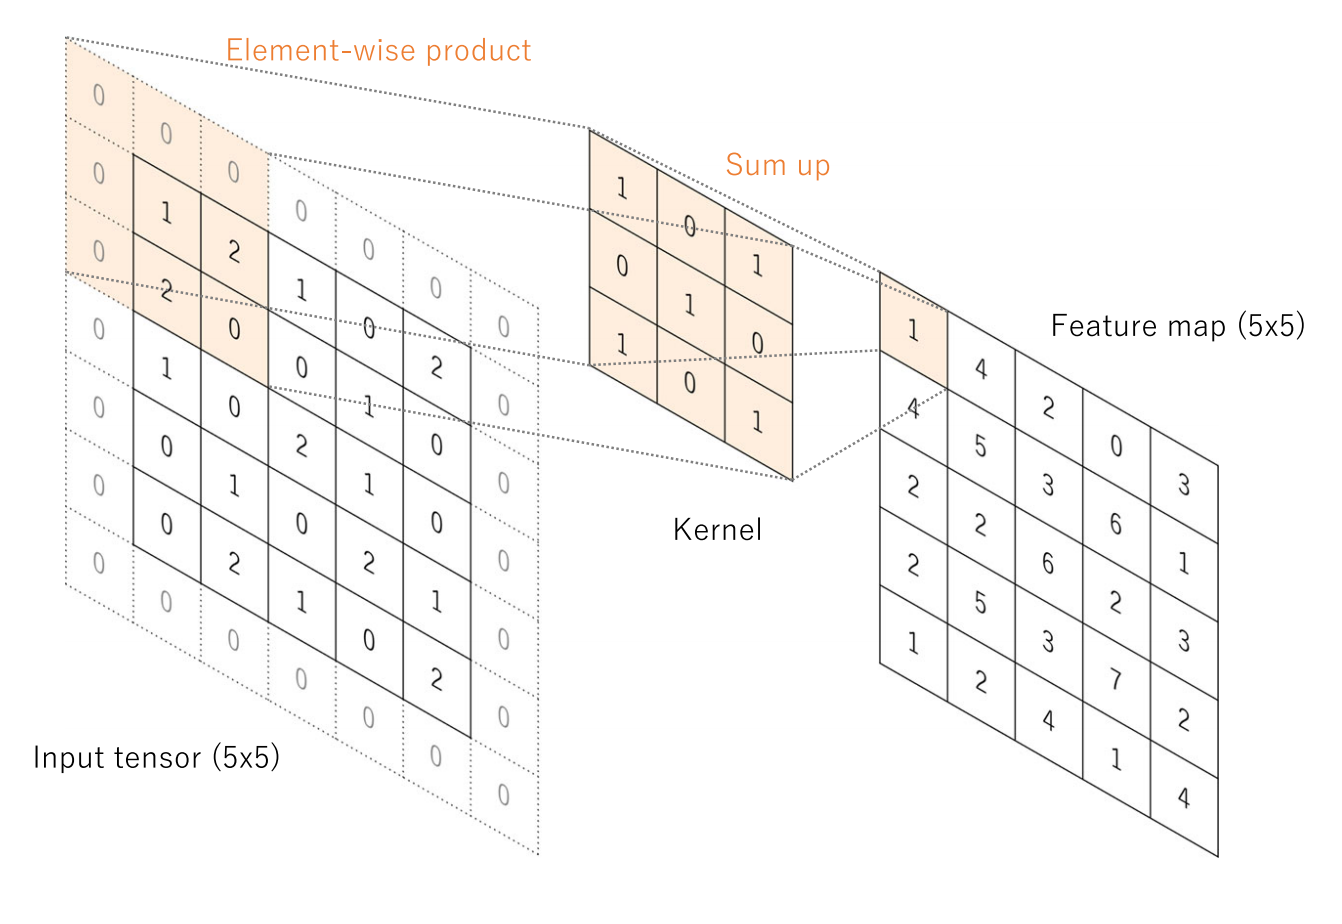
\includegraphics[scale = 0.25]{images/cnn.png}
    \caption{A convolution operation with zero padding so as to retain in-plane dimensions. Image and caption source: \cite{cnnfig}}.
    \label{fig:cnn}
\end{figure}

To make this more formal, consider this formalisation from \cite{csmlnotes}:

Suppose we apply $F_{l+1}$ filters, each of shape $W_f \times H_f \times F_t$, then we can write the entries $z_{i',j',f'}^{l+1}$ in this layer as follows (we assume no zero-padding and stride of 1 in each direction):



 \[z_{i',j',f'}^{l+1} = b^{l+1,f'} + \sum_{i=1}^{W_{f'}}\sum_{j=1}^{H_{f'}}\sum_{f=1}^{F_l}a^l_{i'+i-1,j'+j-1,f} w^{l+1,f'}_{i,j,f}
 \]
 
 Above $w^{l+1,f'}_{i,j,f}$ is the parameter for the $f$'th filter between layers $l$ and $l+1$ indexed by $(i,j,f)$ \cite{csmlnotes}.
 
 
 
Other operations, such as pooling, can be used in a CNN. \textit{pooling} refers to the idea of reducing the size of a tensor (usually after a convolutional layer) using a mathematical operation \cite{cnn}.

\subsubsection{Recurrent Neural Networks}
Recurrent Neural Networks (RNNs) are a class of neural network that is able to ``remember'' previous inputs using an internal state \cite{rnn}, allowing it to deal with sequential inputs (unlike a standard neural network which does not maintain an internal state). For long time-series data an RNN can suffer from the \textbf{vanishing gradient problem} \cite{rnn} which occurs when the gradient of the loss function approaches zero, thus reducing the changes made to weights and severely limits its ability to train. 

A solution for this problem in RNNs is to use a Gated Recurrent Unit (GRU) \cite{gru} which have operations update-gate and reset-gate which are used to filter the amount of passed information to consider. 

Another popular architecture is the LSTM \cite{lstm}, which builds upon the GRU architecture by providing a forget gate, which regulates the amount of information to be ``forgotten'', and an output gate which decides on the next hidden state \cite{lstm}.

LSTMs and GRUs have both exhibited similar performance in natural language processing tasks \cite{lstmvsgru}, so we will only consider the use of GRU-cells in the architectures of this project.

Figure \ref{fig:rnn} shows the of the LSTM and GRU architectures.

\begin{figure}
    \centering
    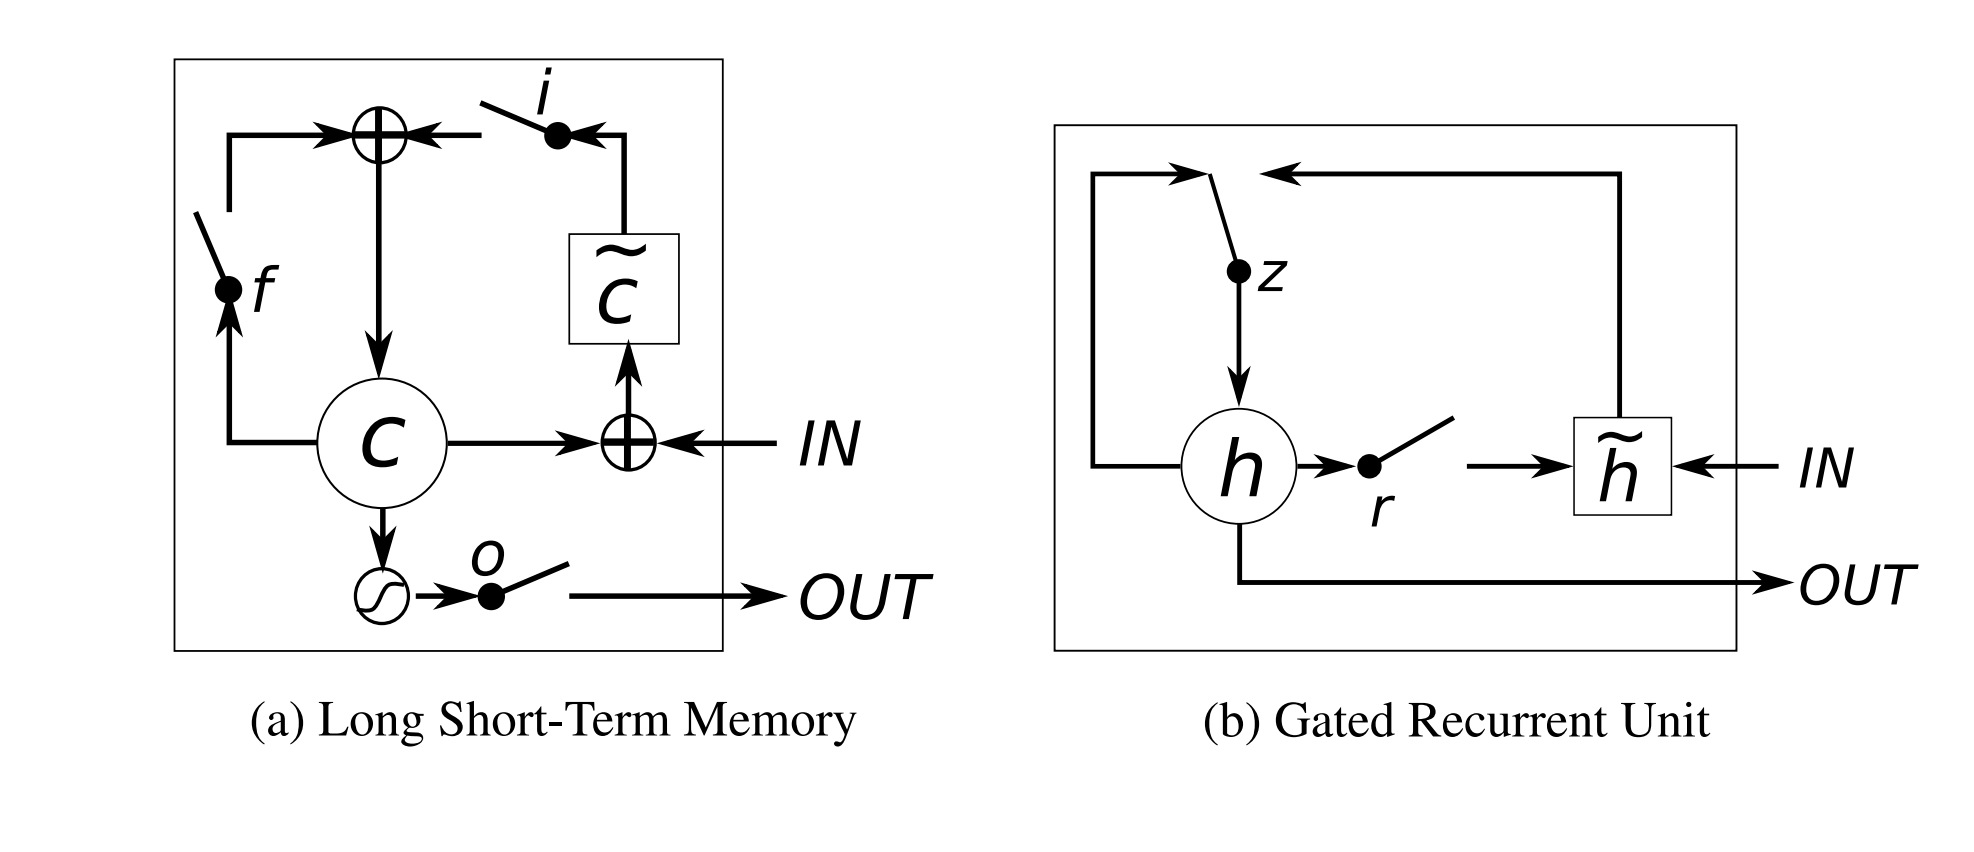
\includegraphics[scale = 0.2]{images/rnn.png}
    \caption{Illustration of (a) LSTM and (b) gated recurrent units. (a) i, f and o are the input, forget and output gates, respectively. c and \~c denote the memory cell and the new memory cell content. (b) r and z are the reset and update gates, and h and \~h are the activation and the candidate activation. Image and caption source: \cite{rnn}.}.
    \label{fig:rnn}
\end{figure}

\subsection{Deep Reinforcement Learning}

Deep RL refers to the use of neural networks within an RL algorithm to approximate some function. In the case of Q-learning in the previous section, a neural network can be used to approximate the state-action value function, $Q$. This modified algorithm is called deep Q-learning (DQN) \cite{dqn}.

In DQN, the neural network eliminates the need for storing a Q-table, significantly reducing the memory requirements. The neural network is better able to approximate state-action values that have not been seen before (but may be similar to those observed previously), allowing for better performance.

Experience replay \cite{expeirnecereplay} is the technique of storing the agent's experiences at each timestep ($e_t = (s_t, a_t, r_t, s_{t+1})$) in a dataset $D = e_1..., e_N$ called the replay memory \cite{dqn}.

As described in \cite{qmixcite}, the weights and biases of the network are learnt by sampling batches of the replay memory and minimising the \textit{TD error}:

\[\mathscr{L}(\theta)=\sum_{i=1}^{b}[(y_i^{DQN}-Q(s,a;\theta))^2]\]

where $y^{DQN}=r+\gamma \max_{a'}Q(s',a';\theta^-)$ ($\theta^-$ are the parameters for a \textit{target network} that are updated using $\theta$ periodically) \cite{qmixcite}.



\subsection{Multi-Agent Reinforcement Learning}
Multi-Agent Reinforcement Learning (MARL) is the process of learning policies for multiple co-operative (or adversarial) agents interacting in the same environment. In this project, we only consider co-operative agents. One paradigm of MARL is \textit{centralised learning with decentralised execution}, which allows for a single controller (which has access to the global state) to coordinate the learning of all agents, while during execution each agent operates independently using its learned policy.

\subsubsection{The StarCraft Multi-Agent Challenge}

Recent progress in MARL has seen the need for a benchmark of performance, including a specific environment and method for quantifying performance. A popular benchmark fitting this description is the StarCraft Multi-Agent Challenge (SMAC) \cite{smac}. SMAC is based upon the science-fiction real-time strategy game StarCraft II in which teams of various units battle against one another. Although the game is far more complex than this (with resource management, buildings as well as other considerations), SMAC only considers situations of this form. Each unit is controlled by a single agent, and SMAC specifies various maps (the number and type of the units on either team) as well as allowing control over the difficulty of the AI controlling the opposing team. 


In SMAC (and in this project) we consider the following unit types:

\vspace{3mm}
\begin{center}
\begin{tabular}{ |p{2.5cm}||p{6.6cm}|  }
 \hline
 \centering Unit Type& \centering Description \tabularnewline
 \hline
 \centering Marine   & A cheap, all-purpose infantry unit\tabularnewline
 \hline
 \centering Stalker   & A fast moving ranged unit\tabularnewline
 \hline
 \centering Zealot   &  A strong brute-force unit\tabularnewline
 \hline
 
\end{tabular}
\end{center}
\vspace{3mm}


\subsubsection{Dec-POMDPs}
A decentralised partially observable Markov decision process (dec-POMDP) is an extension of a regular MDP for use in multi-agent reinforcement learning. 

As described in \cite{dec-pomdp}, we can define a dec-POMDP as follows:
\begin{definition}\textbf{\normalfont{\cite{dec-pomdp}}}{ (Dec-POMDP)}
A decentralised partially observable Markov decision
process is defined as a tuple $\mathscr{M} = \langle \mathbb{D,S,A},T,\mathbb{O},O,R,b_0\rangle$, where
\begin{itemize}
    \item $\mathbb{D}=\{1,...,n\}$ is the set of n agents.
    \item $\mathbb{S}$ is a (finite) set of states.
    \item $\mathbb{A}$ is the set of joint actions.
    \item $T$ is the transition probability function.
    \item $\mathbb{O}$ is the set of joint observations.
    \item $O$ is the observation probability function.
    \item $R$ is the immediate reward function.
    \item $b_0$ is the initial state distribution at time $t = 0$.
    
\end{itemize}
\end{definition}

At each time step (with the environment in state $s \in \mathbb{S}$), each agent $d \in \mathbb{D}$ will choose an action $a^d$ (to form the joint action $\textbf{a} \in \mathbb{A}$) and will transition to a new state $s'$ with probability $T(s'|s,\textbf{a})$. Each agent will receive the reward $R(s, \textbf{a})$. Individual observations $o^d$ are made by each agent to form the joint observation $\textbf{o} \in \mathbb{O}$. A joint observation \textbf{o} occurs with probability $O(\textbf{o})$. There is an action-observation history $\tau^d \in (\mathbb{A} \times \mathbb{O})^*$ for each agent $d \in \mathbb{D}$. This conditions a stochastic policy $\pi^d(a^d|\tau^d) : (\mathbb{A} \times \mathbb{O})^* \times \mathbb{A} \to [0, 1]$. Intuitively, the policy $\pi^d$ gives the probability that a particular action $a^d$ is taken, given an action-observation history $\tau^d$, for agent $d$.

\subsubsection{Independent Q-Learning}
Independent Q-learning \cite{IQL} is a simple extension of Q-learning to the multi-agent setting. The problem is decomposed into multiple agents, each employing Q-learning independently, sharing the same environment. Although this technique does not account for the non-stationarity of sharing the same environment, it is surprisingly effective in practise \cite{iqlisgood}. 


\subsubsection{Value Decomposition Networks}
Value Decomposition Networks \cite{vdn} (VDN), by contrast, aim to learn a joint action-value function

\[Q_{tot}(\boldsymbol{\tau}, \textbf{a}) = \sum_{i=1}^{n} Q_i(\tau^i,a^i;\theta^i) \]

where $\boldsymbol{\tau}$ is the joint observation history, $\textbf{a}$ is the joint action, $Q_i$ is the $Q$ function for agent $i$ and $\theta^i$ are the parameters for agent $i$'s network.

Q is then learnt in the same way as DQN, but during execution this policy is very easy to decentralise (each agent chooses greedily with respect to its own $Q_i$).

During execution, each agent can simply use its own $Q$-network it trained during training. This follows the \textit{centralised learning with decentralised execution} paradigm.

\subsubsection{QMIX}
QMIX is a state-of-the-art deep MARL algorithm that lies between the extremes of IQL and centralised Q-learning \cite{qmixcite}. Instead of requiring the decentralised policies be consistent with the centralised counterpart, as in VDN, all that we require in this section is that a global argmax performed on $Q_{tot}$ yields
the same result as a set of individual argmax operations
performed on each $Q_a$:

\[\argmax_{\textbf{a}}Q_{tot}(\boldsymbol{\tau},\textbf{a}) = \begin{bmatrix}
        \argmax_{a^1}Q_1(\tau^1,a^1) \\
        \vdots\\
        \argmax_{a^n}Q_n(\tau^n,a^n)
    \end{bmatrix}\]


As a consequence of this constraint, as in VDN, an agent can execute in a decentralised fashion simply by choosing $a$ greedily according to its Q-value.




QMIX represents $Q_{tot}$ using an architecture
consisting of agent networks, a mixing network, and a set
of hypernetworks \cite{hypernetworks} \cite{qmixcite}. Each agent has its own deep recurrent Q-network (DRQN) \cite{dqrn},the outputs of which are fed into the mixing network: a feed-forward neural network that mixes them
monotonically, producing the values of $Q_{tot}$ \cite{qmixcite}. The weights of the mixing network are produced by separate hypernetworks \cite{qmixcite}.

An overview of the networks can be seen in figure \ref{fig:qmix}, but further details can be found in \cite{qmixcite}.

\begin{figure}
    \centering
    \hbox{\hspace{-2.5em}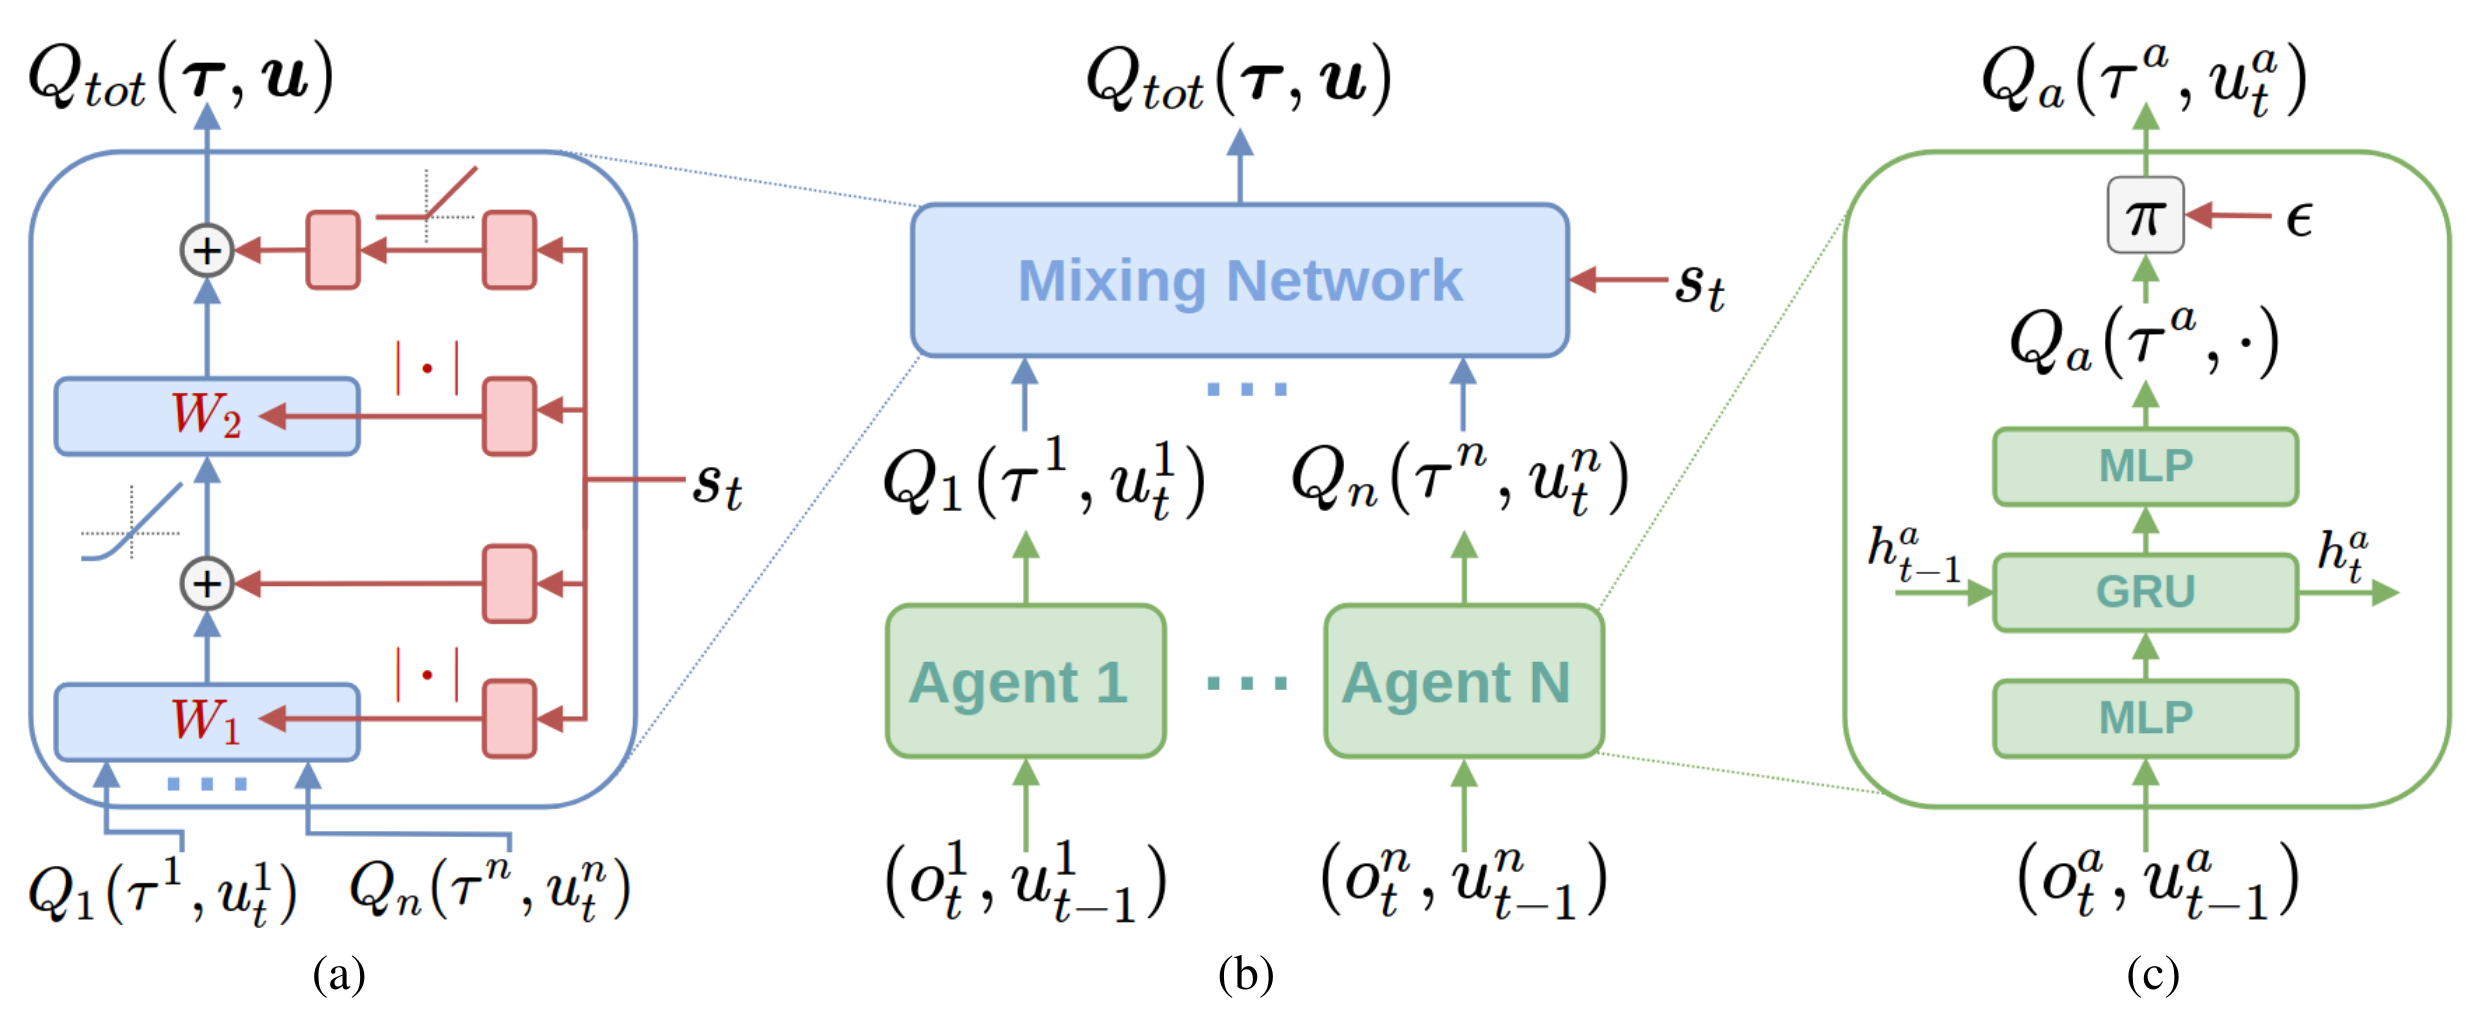
\includegraphics[scale = 0.18]{images/qmix.png}}
    \caption{(a) Mixing network structure. In red are the hypernetworks that produce the weights and biases for mixing network layers shown
in blue. (b) The overall QMIX architecture. (c) Agent network structure. Image and caption source: \cite{qmixcite}.}
    \label{fig:qmix}
\end{figure}





QMIX is trained in the same way as in DQN, replacing $Q$ with $Q_{tot}$.



\section{Methodology}
As described in section 1.2, the PyMarl framework is a collection of various multi-agent RL algorithms. It uses the PySC2 library \cite{pysc2}, an open source StarCraft II environment that is optimised for RL agents, which passes observations as lists of units and their properties. In the PyMarl framework, we must define an agent network (which is a neural network architecture that each agent uses to determine $Q$-values) and a mixing network, which takes each agent's $Q$-value to produce a total $Q$-value, $Q_{total}$. Note the difference between an agent and an agent network: an agent is one of many actors within the multi-agent system, whereas the agent network is the neural network architecture that makes up the $Q$-value function of each agent. Furthermore, every agent in the environment uses the same neural network, and shares the network weights. This decreases the space required. We will fix the mixing network to either VDN or QMIX, as these have been shown to have good performance in previous tests. 

The agent networks are implemented in Python using the PyTorch framework \cite{pytorch}, as this allows for great flexibility in building neural networks, as well as allowing for the use of the graphical processing unit (GPU) for training, specifically it offers strong tensor computation compatible with the GPU.

The agent network takes the form of a neural network to approximate the state-value function, which takes an input (a tensor) consisting of an observation (and possibly a particular action). Due to PyTorch's ability to batch process multiple inputs through a neural network, we are able to combine the inputs for every agent into a single tensor, and process this for efficiency. Concretely, if there are $n$ agents and each observation has size $o$, then the input tensor has shape $(n, o)$, while the output tensor of $Q$ values has size $(n, a)$, where $a$ is the number of actions (since we have an output for each available action, representing its corresponding $Q$-value). Conversely, if the agent network takes actions as input also (and gives a single $Q$ value as output), then the input tensor has shape $(n \times a, o)$ and the output tensor has shape $(n \times a, 1)$.

As described in section 2.6, the $Q$-value for each agent is fed into a mixing network (e.g. QMIX or VDN), to determine $Q_{total}$. Using backpropagation we can train the entire network, including the mixing network.

Several approaches have been taken to design the agent networks, including various combinations of convolutional and recurrent neural networks, as well as different representations of both observations and actions. Here we discuss these approaches in detail, as well as considering the challenges associated with each method.



To train the agent networks, a server of Nvidia RTX 2080 TI GPUs is used which provides a large amount of computational power. The parallel computing platform CUDA \cite{cuda} is also employed to run experiments on the server.




\subsection{Recurrent Neural Network Agents}


The first agent networks we will explore are simple RNN agents. RNNs are generally well suited to this task due to their ability to store past information (such as the enemy most recently attacked or where it has moved from) in an internal state. This enables the agent to have more historical context to its inputs and own decisions.

We first consider an RNN agent network that takes observations (consisting of surrounding enemies/allies, its own health, its agent ID etc.) as inputs, and outputs a $Q$ value for each available action. The observations are passed through a fully connected linear layer before a rectified linear unit (ReLU) as the network non-linearity. We use ReLU as opposed to tanh or sigmoid as ReLU does not suffer as greatly from the vanishing gradient problem, as it only saturates in one direction \cite{relu}. The next layer is a GRU-cell. Finally, a fully-connected linear layer is used to provide the output $Q$-values.

If an action is not possible (for example, another unit is blocking its path, so the agent may not move in that direction), then we set its corresponding $Q$ value to $-\infty$ after the feedforward (to prevent it from being chosen).

This particular agent network is the standard network implemented in the PyMarl framework. It is relatively simple, but performs fairly well in practice. It will act as a benchmark for other agent networks using various other approaches.

Its architecture is shown in figure \ref{fig:rnn_agent_diagram}.

\begin{figure}
    \centering
    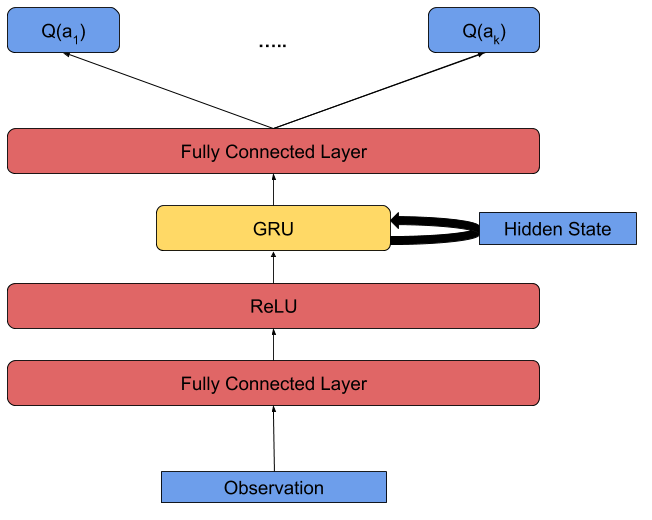
\includegraphics[scale=0.45]{images/agent_diagrams/rnn_agent_diagram.png}
    \caption{The standard \textit{rnn} architecture.}
    \label{fig:rnn_agent_diagram}
\end{figure}






\subsection{Grid Representation of Observations and Actions}

A relatively simple way to abstract an observation of a particular agent is to generate a grid (with the agent at the centre) with various channels containing relevant features, with each cell representing a location in this agent's field of view. The features may include whether a particular cell contains an ally or an enemy unit (or neither), the health of a unit and the type of a unit (Marine, Zealot etc.). 

We are also able to represent actions in a similar way. There are two main types of action we wish to consider: movement and attack. Therefore, two channels in the action grid are required to differentiate between the two. We can place a value of $1$ in the cell north, south, east or west of the agent we are considering (in the movement channel) to represent a movement in the respective direction. All other values will be zero, as we are only considering one action at a time. For attack, we place a value in the cell of the unit we are wanting to attack (in the attack channel), again with zeroes in all other cells.

In both of these cases, the grids are three dimensional tensors (in the PyTorch framework).

The reason for these style of observations is to allow for the use of convolutional neural networks to better find patterns in the graphical representation of the environment, as we will explore in the following section.

\subsubsection{Observation and Action Decoders}

Some key pieces of engineering to allow for the use of grid-based actions and observations are the action encoder and observation decoder. 

The action encoder turns StarCraft II actions (one-hot encoding) into grid actions (with 2 channels for movement and attack). In the action grid, the central cell represents the agent with respect to its field of view. If the action is a movement action, then a 1 is filled in the adjacent north, south, east or west cell (depending on which direction the action is) in the movement channel. All other cells are left as 0. If the action is an attack action, then a 1 is filled in the cell in which the unit to attack is occupying, in the attack channel. Again, all other cells remain as 0. 

The observation encoder turns StarCraft II (one dimensional) observations into grid observations. The centre of the grid represents the agents location, and observations are represented by filling the relevant cell in a specific channel with the necessary observation information, while all other cells have value 0. For example, the health observation sets cells representing unit locations (in the health channel) to the health of those units. 

Note that both encoders do not have any learnt parameters, and are simply used to prepare the inputs before they are passed into the agent network.

\subsubsection{Convolutional Neural Network Agents}

A possible way to enhance the performance of the simple RNN-based agent networks is to include convolutional layers in the network. This allows the agent network to make stronger deductions about the relations between entities in each observation, and recognise patterns that would otherwise not be noticed, especially if observations and actions are represented as images (grid-based). 

The convolutional layers will form a convolutional encoder, that was originally shown to be successful in \cite{ddpg}, which explored the use of deep deterministic policy gradients (DDPG). The encoder is simply three convolutional layers, which have 32 filters each and no pooling. After each convolutional layer, an exponential linear unit (ELU) is used as the activation function.

Clevert et al. \cite{elu} give the following advantages of the ELU activation function: ``In contrast to rectified linear units (ReLUs), ELUs can output negative values which allows them to push mean unit activations closer to zero like batch normalisation but with lower computational complexity. Mean shifts toward zero speed up learning by bringing the normal gradient closer to the unit natural gradient because of a reduced bias shift effect.''


We first consider a simple agent network using this convolutional encoder (as well as a GRU-cell, to allow for the same power as the previous RNNs). We first feed the grid-based observation into the convolutional encoder, before flattening the output into a 1-dimensional tensor. We do this to be able to concatenate the 1-dimensional observation information (agent identifier, last action performed etc.). The next layer is a fully connected linear layer, before a rectified linear unit as the activation function. What follows is a GRU-cell and another fully-connected layer, which outputs a Q-value for each possible action. Intuitively, the convolutional encoder captures various information about the relation between entities in the observation, while the multiple fully-connected layers extract this information into the Q-values. The GRU-cell allows for the network to use information about the historical time-series data, to give an even more informed result. We shall refer to this agent network as \textit{conv}. The architecture of this agent network is shown in figure \ref{fig:conv_agent_diagram}

\begin{figure}
    \centering
    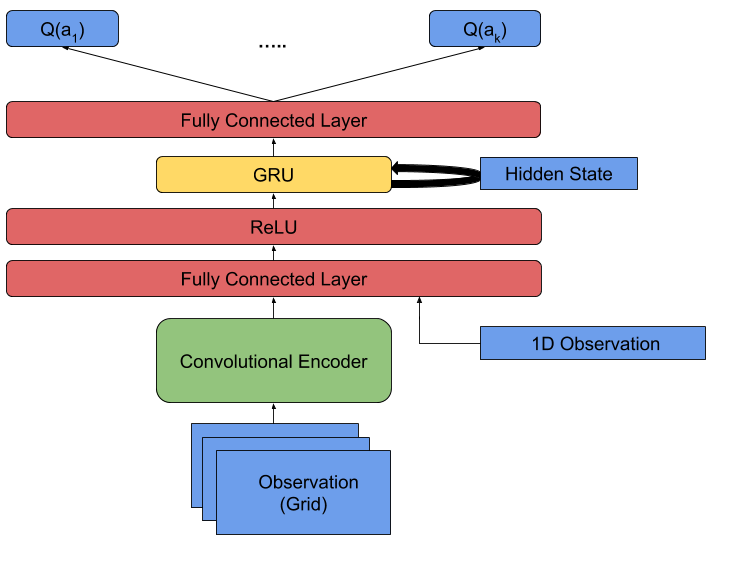
\includegraphics[scale=0.45]{images/agent_diagrams/rnn_conv_dpdpg_agent_diagram.png}
    \caption{The \textit{conv} architecture.}
    \label{fig:conv_agent_diagram}
\end{figure}

We can also experiment with the idea of using a candidate action as an input in order to output a single $Q$-value (for that observation-action pair), rather than simply have a $Q$-value for each possible action. This yields a new agent network, which inputs grid observations into the convolutional encoder as normal, but concatenates a candidate action onto the 1-dimensional encoded observation. The layers are the same as in conv, except that the last fully-connected linear layer has a single output, for the $Q$-value corresponding to the particular observation and action pair. We shall refer to this agent network architecture as \textit{conv\_input\_flat}. 

Passing actions as inputs in this way changes the shape of the network, with more neurons at the input (to deal with the action), and less neurons at the output (we no longer output a $Q$ value for each action). This may have implications to the speed of training and overall performance, and is therefore important to experiment with. 

The architecture is shown in figure \ref{fig:conv_input_flat_diagram}.

\begin{figure}
    \centering
    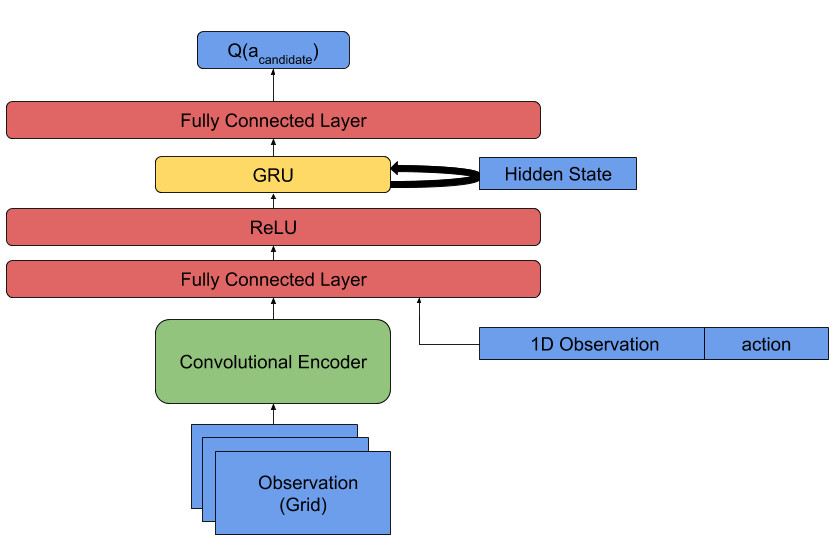
\includegraphics[scale=0.45]{images/agent_diagrams/rnn_mathias_agent_diagram.png}
    \caption{The \textit{conv\_input\_flat} architecture.}
    \label{fig:conv_input_flat_diagram}
\end{figure}


The previous two agent networks’ convolutional encoders do not encode any information about the possible actions, only the observations. Therefore, a possible change that can be made is to somehow include the actions (in their grid-based representations) as an input into the encoder. This requires us to input actions into the network first, and receive a single Q-value for that particular observation and action pair, rather than receive a Q-value for each possible action. As described before, actions are represented in a similar way to observations, but with just 2 channels (movement and attack), with a single 1 in a cell to represent movement (or attack) to a particular location in the agent's field of view. The architecture of this agent network is similar to that of the \textit{conv} architecture, but the action grid representation for a single possible action is concatenated to an observation in its grid representation, and then is fed forward through the network as normal. Therefore, the entire input constitutes of a series of observation-action pairs (in this concatenated grid form), one for each observation and possible action. We also only have a single output from the last fully connected linear layer, representing the Q-value of that particular observation-action pair. This agent network architecture will be referred to as \textit{conv\_input\_grid}.

The architecture can be seen in figure \ref{fig:conv_input_grid_agent_diagram}.

\begin{figure}
    \centering
    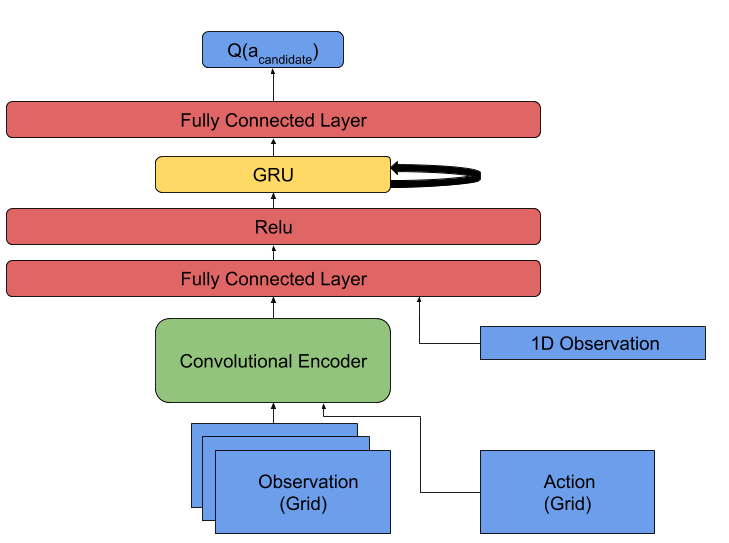
\includegraphics[scale=0.45]{images/agent_diagrams/rnn_conv_ddpg_input_grid_agent_diagram.png}
    \caption{The \textit{conv\_input\_grid} architecture.}
    \label{fig:conv_input_grid_agent_diagram}
\end{figure}





\subsection{Grid Size}

We are able to change the ``resolution'' of the observation (and action grid) by changing the width and height of the grid. The grid always covers only the field of view of the agent, but the number of cells in the grid (i.e. the ``resolution'') can be changed.  A larger number of cells in the grid gives a greater amount of detail, but also a greater amount of computation will be required and more sparse images will be generated. Therefore, a balance has to be made. This will form a large part of the experiments for these agent networks.





\subsection{Problems Encountered}
In the implementation of these agent networks, there were multiple challenges to overcome. We briefly overview the most prominent in the following sections.

\subsubsection{Multiple Occupancy}
Observation and available action information can be lost when multiple units are close enough to occupy the same cell in the grid representation: an agent would be disadvantaged in cases where the superior actions differ depending on the number of units in a specific location. This is especially apparent with smaller grid resolutions. A simple way to mitigate this effect is to alter the observation to distribute the location of units to neighbouring cells in the case of multiple occupancy. This can be done with a simple randomised algorithm, Algorithm \ref{multipleoccupancyalg} details the procedure.

\begin{algorithm}
    \caption{ResolvingMultiple Occupancy}
    \label{multipleoccupancyalg}
    \begin{algorithmic}
        \Procedure{ResolveMultipleOccupancy}{}
        \While{there is some cell containing multiple units}
        \State c = a cell with more than one unit
        \State unit = arbitrary unit in cell c
        \State c' = random cell adjacent to c
        \State move unit from c to c'
        \EndWhile
        
        \EndProcedure
      
        
        
    \end{algorithmic}
    
\end{algorithm}

\subsubsection{Memory Usage}

Memory usage was large for the architectures using grid representation of observations or actions, especially on maps with more than 10 or more units. This can be explained by the sparsity of the grid tensors: there are only $n$ cells with non-zero values, where $n$ is the total number of units in the map, compared to a total of $W \times H \times C$ cells ($W$,$H$, $C$ being the width, height and number of channels in the grid respectively) is extremely sparse. Each cell is a 4-byte float, thus a single grid representation of observations and action, of size $12 \times 12$, with 3 observation channels and 2 action channels, takes up $4 \times 12 \times 12 \times 5 = 2880$ bytes. 

The replay buffer contains the most recent 5000 episodes, with each episode being at least 100 timesteps. We have an observation for each agent and each available action, so there are $5000 \times 100 \times 3 \times 9 = 1.35 \times 10^7$ such grids in the replay buffer. This gives a total size of $1.35 \times 10^7 * 2880 \text{ bytes} \approx 38.9Gb$, which is far too large for RAM, let alone GPU memory.


A solution to this problem is to use a compressed representation: storing the observations and actions as lists in the buffer, and decompressing them into the grid representation ``on-the-fly''. This method proved successful and allowed the replay buffer to be stored easily in RAM, albeit with a computation time trade-off

However, on larger grid sizes (e.g $24\times24$) the batch was still too larger. A standard batch size of 32 \cite{smac} gives an average total size of at least $500Mb$, but this can easily become too large for the GPU memory. 

A smaller batch size is therefore used for larger grid sizes (above $12 \times 12$). However, the batch size can have an impact on training performance: a larger batch size generally decreases the variance of the estimates of $Q$-values, allowing for more consistent gradient descent traversals. However, a lower batch size can introduce more noise in the sampling, and allows for escaping local minima, as well as avoiding overfitting.

With these considerations, in situations where memory usage is high, it is generally advisable for the batch size to be as large as possible before memory usage becomes too high. Testing found the following batch sizes effective with a 5Gb GPU memory limit for various grid sizes.

\vspace{3mm}
\begin{center}
\begin{tabular}{ |p{1.8cm}||p{1.8cm}|p{7.5cm}|  }
 \hline
 Grid Size& batch\_size& Approximate Memory Usage During Training\\
 \hline
 \centering 6x6   & \centering 32 & \centering2.0Gb\tabularnewline
 \hline \centering 12x12   & \centering 32 & \centering4.5Gb\tabularnewline
 \hline
 \centering 18x18   & \centering 16 & \centering5.0Gb\tabularnewline
 \hline
 \centering 24x24   & \centering12 & \centering5.5Gb\tabularnewline
 \hline
\end{tabular}
\end{center}
\vspace{3mm}












\subsection{StarCraft Task Invariant Architectures}
Architectures that use actions or agent IDs (in their standard representations) as inputs or outputs are not invariant to the task in StarCraft. This is because a different map has a different number units, and thus more enemies to attack and more agent IDs to assign. This requires a larger one-hot encoding, so the architecture is changed.


We hypothesise that architectures independent of task can generalise well over tasks. Grid-representation of observations and actions get us closer to this invariance, as actions are no longer one-hot encoded, but are represented in a universal grid form. Furthermore, this representation is well-suited to generalising over tasks as agent interactions depend on spatial arrangement. 

The architecture closest to task invariance is conv\_input\_grid, since it uses grid actions. Furthermore, in order to make it fully invariant to tasks, we simply need to remove the input for the agent ID and use the VDN mixing network (QMIX requires an input for each agent, so is not invariant, but the VDN network does not have this problem). We hypothesise that the observation and action encodings is rich enough to distinguish between agents, and thus this input is not necessary. 


Therefore, by removing this input from the conv \_input\_grid architecture, we produce our final architecture, conv\_input\_grid\_no\_id, which (when used with the VDN mixing network) is task invariant.




A huge advantage to network architectures which are invariant to the task is the ability for transfer learning. Due to the similarity of the tasks (enabled by the partial observability), it is extremely useful to train on smaller, simpler tasks before attempting to learn on more complex tasks with a far greater state space. This has the effect of speeding up training time and even increasing final performance \cite{curriculum}.





\section{Experiments}
To evaluate the performance of each architecture, a number of experiments are carried out. These experiments take the form of training the networks on a particular map, and testing the model every so often by measuring the win rate against the built-in AI.

\subsection{Experimental Setup}

The particular maps contain a set of units for either team, with one team composed of the agents, and the other controlled by the built-in AI on ``very hard'' difficulty (which is the hardest built-in non-cheating AI difficulty). This is the same difficulty that is used in \cite{smac}.

The specific maps we will use in experiments are shown in the table below.

\vspace{3mm}
\begin{tabular}{ |p{2.5cm}||p{6.6cm}|  }
 \hline
 \centering Map Name& \centering Description\tabularnewline
 \hline
 \centering 3m   & 3 Marines on each team\\
 \hline
 \centering 5m   & 5 Marines on each team\\
 \hline
 \centering 8m   & 8 Marines on each team\\
 \hline
 \centering 2s3z   & 2 Stalkers and 3 Zealots on each team\\
 \hline
 \centering 3s5z   & 3 Stalkers and 5 Zealots on each team\\
 \hline
 
\end{tabular}
\vspace{3mm}

The experimental setup is the same as that of \cite{smac}: ``Exploration is performed during training using independent $\epsilon$-greedy action selection, where each agent $a$ performs $\epsilon$-greedy action selection over its own $Q_a$. Throughout the training, we anneal linearly from 1.0 to 0.05 over 50,000 time steps and keep it constant for the rest of the learning. We set $\gamma= 0.99$ for all experiments. The replay buffer contains the most recent 5000 episodes.  We sample batches of 32 [dependent on grid size] episodes uniformly from the replay buffer, and train on fully unrolled episodes, performing a single gradient descent step after every episode.'' 

The training is paused every 20,000 timesteps, during which 32 test episodes are run with agents performing action selection greedily in a decentralised fashion. The percentage of episodes where the agents defeat all enemy units within the permitted time limit is referred to as the \textit{test win rate}.

Each agent network is trained using 5 distinct random seeds (which are used for all random operations) to validate the replicability of the results. Furthermore, we calculate the mean and standard deviation of the test win rate of these 5 runs.

\subsection{Baseline Experiments}

The first set of experiments will evaluate the performance of each candidate architecture on various maps. Both the QMIX and VDN mixing networks will be used to allow us to compare the performance of each candidate architecture using each mixing network. The grid size is set to $12\times12$, as this showed good potential in early tests, while minimising memory usage.


\subsubsection{Baseline Experiments on 3m}

Firstly we shall test the performance of the candidate architectures on the 3m map. We can see the performance of each architecture in figure \ref{fig:3m_all}. 

Using the VDN mixing network, all architectures exhibit excellent performance, reaching a near perfect win rate within just 500,000 timesteps with low variance, matching the performance of the standard \textbf{RNN} architecture.

Using the QMIX mixing network, every architecture also performed very well on the 3m map, again matching the performance of the standard \textbf{RNN} architecture. 

The fact that the more complex grid-based architectures did not have greater performance than the standard \textbf{RNN} architecture in this map is interesting, but likely explained by the simplicity of the 3m map: a convolutional encoder and grid representation is simply not needed for a map with this few (identical) units.

\begin{figure}[h]
    \centering
    \hbox{\hspace{-6.35em}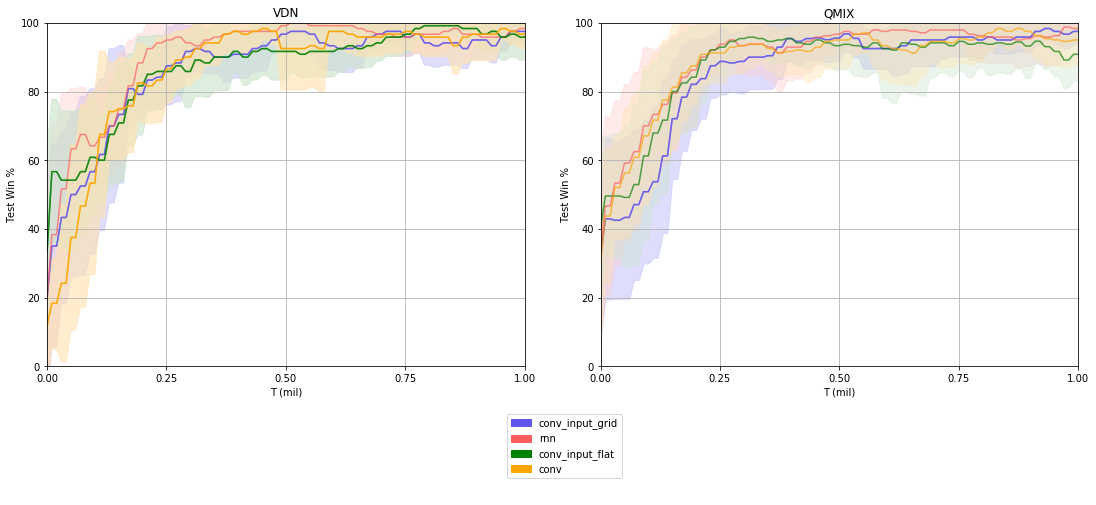
\includegraphics[width=1.34\textwidth]{images/graphs/all3m.png}}
    \caption{Mean test win rates of different architectures on the 3m map with both the VDN and QMIX mixing networks. The shaded region shows one standard deviation above and below the mean. We can see that each architecture performs similarly, exhibiting very high performance using both VDN and QMIX .}
    \label{fig:3m_all}
\end{figure}

\subsubsection{Baseline Experiments on 2s3z}
We now perform the same experiments on the 2s3z map. The results of these experiments (for both the VDN and QMIX mixing networks) can be seen in figure \ref{fig:2s3z_all}.

Using the VDN mixing network, we can see both the \textbf{conv} and \textbf{conv\_input\_flat} architectures exhibit lesser performance when compared to the standard \textbf{RNN} architecture, while the \textbf{conv\_input\_grid} architecture matches its performance. This suggests that grid-based actions as inputs are more useful to an agent than grid-based observations, and provide a superior insight into its environment.


Using the QMIX mixing network, performance was higher on all architectures (when compared to the VDN mixing network): each exhibited a large limit win rate and fast convergence. However, we clearly see that both the \textbf{conv} and \textbf{conv\_input\_flat} architectures under-performed compared to the standard \textbf{RNN} network. This suggests that, in a more complex map with multiple types of units (such as 2s3z), if an architecture is using a convolutional encoder for grid-based observations then it needs grid-based actions as inputs to be effective. 

There was increased variance in the performance on the 2s3z map when compared to the 3m map. This is likely due to the grid representation of observations, and the different numbers of units: the relationships between the agents (and enemies) is harder to capture on this map.

\begin{figure}[h]
    \centering
    \hbox{\hspace{-6.35em}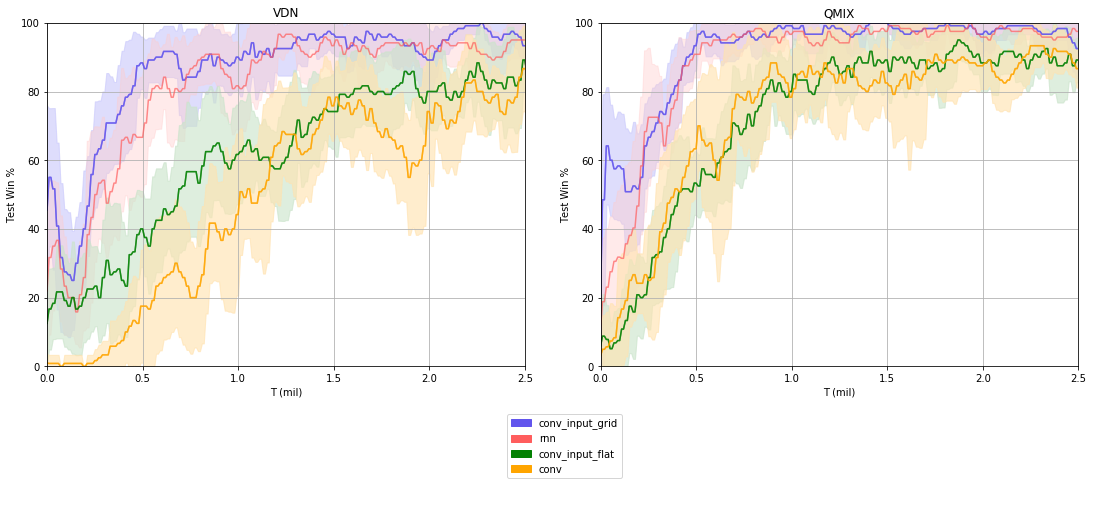
\includegraphics[width=1.34\textwidth]{images/graphs/all2s3z.png}}
    \caption{Mean test win rates of different architectures on the 2s3z map using both the VDN and QMIX mixing networks. The shaded region shows one standard deviation above and below the mean. The \textbf{conv\_input\_grid} and \textbf{RNN} architectures perform similarly and are clearly superior to the other architectures.}
    \label{fig:2s3z_all}
\end{figure}





\subsection{Experiments On Different Grid Sizes}
In this section we experiment with different grid sizes for the inputs of \textbf{conv\_input\_grid} (both the observations and actions as inputs). A trade-off is made between the simplicity of a small grid (which has a smaller network that can train more quickly) and the level of detail that can be achieved with a larger grid, allowing for greater spatial relationships to be made between the units.

The experiments will be performed using the same set up as before, and will take place on the 2s3z map, as this includes units of different types.



The grid sizes tested are $6\times6$, $12\times12$, $18\times18$ and $24\times24$. This is because the convolutional encoder kernels (of size $3\times3$) are simply too large for an input of size smaller than $6\times6$, and recent tests show that grids larger than $24\times24$ run out of memory, even with small batch sizes. As described in section 3.3.2, some simple tests were run to find the optimal batch sizes for the different sizes of grid observations. Every other configuration parameter was kept the same for each experiment.





The \textbf{conv\_input\_grid} architecture was the architecture chosen to experiment upon for each of these grid sizes, as it showed very promising performance in the baseline experiments, and uses grid-representation for both observations and actions. The results are shown in figure \ref{fig:gridsizes}.


\begin{figure}
    \centering
    \hbox{\hspace{5em}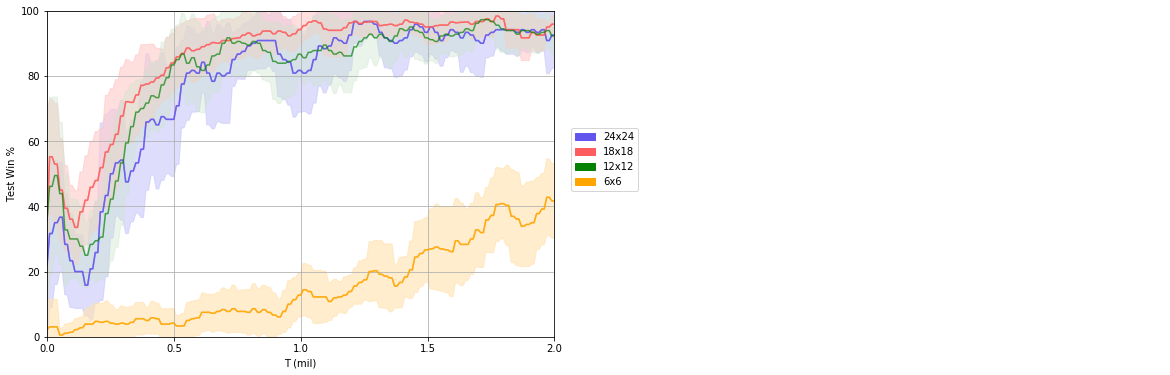
\includegraphics[scale=0.5]{images/graphs/grids.png}}
    \caption{Mean test win rate of the \textbf{conv\_input\_grid} architecture with various grid sizes. The shaded region shows one standard deviation above and below the mean. All tested grid sizes perform well, apart from the $6\times6$ size, which clearly exhibits inferior performance.}
    \label{fig:gridsizes}
\end{figure}

The $12\times12$, $18\times18$ and $24\times24$ grid sizes performed very similarly, each having good performance. Each size has a very large initial rate of learning, reaching around a $50\%$ test win rate very quickly. From here on, each of these grid sizes exhibit a steady increase to its convergence of around a $92\%$ test win rate after 3 million timesteps. The similarity of these results suggest that a grid size of $12 \times 12$ or above is enough to represent the environment effectively.




Clearly, the $6 \times 6$ grid performs very poorly: although some learning can be seen to have taken place, little progress and large variance is still apparent in comparison to the other sizes. This is likely a result of the grid not being able to represent the complexities of the environment well enough: the relations between agents has been abstracted too far away, since 36 cells is not enough to represent this. 

Another suggestion for this lack of performance is the effect of multiple occupancy. On a smaller grid, it is more likely that multiple occupancy will occur, which may have a negative effect on performance, as the observation the agent receives is different from the true observation. In order to see this, we will run a simple test to measure the number of time multiple occupancy occurs over a period of training. Shown in the table below are the average number of cells with multiple occupancy per observation, rounded to two significant figures:


\vspace{3mm}
\begin{center}
\begin{tabular}{ |p{1.8cm}||p{8cm}|  }
 \hline
 \centering Grid Size& \centering Mean Number of Cells With Multiple Occupancy\tabularnewline
 \hline
 \centering $6\times6$   & \centering 0.65\tabularnewline
 \hline
 \centering $12\times12$  & \centering 0.25\tabularnewline
 \hline
 \centering $18\times18$  & \centering 0.18\tabularnewline
 \hline
 \centering $24\times24$   & \centering 0.0026\tabularnewline
 \hline
 
\end{tabular}
\end{center}
\vspace{3mm}


This makes sense, as the probability of two units occupying the same cell in the grid should decrease in an inverse square fashion, which is similar to what we see here. 

Figure \ref{fig:multocc} shows a comparison of performance between the \textbf{conv\_input\_grid} architecture with and without the resolve multiple occupancy (RSO) algorithm, on both the $6\times6$ and $12\times12$ grid sizes. This experiment was performed on the 2s3z map.

\begin{figure}
    \centering
    \hbox{\hspace{5em}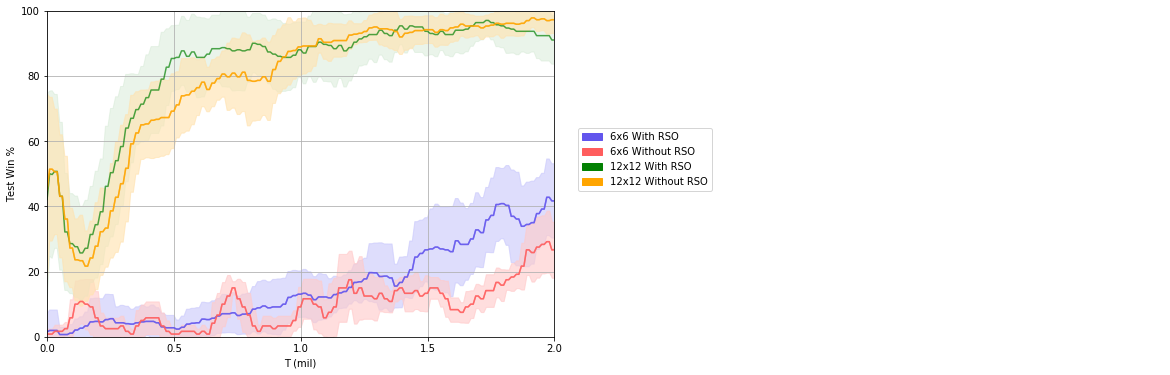
\includegraphics[scale=0.5]{images/graphs/mult_occ.png}}
    \caption{Mean test win rate of the \textbf{conv\_input\_grid} architecture (with various grid sizes) with and without the resolve multiple occupancy (RSO) algorithm. The shaded region shows one standard deviation above and below the mean. RSO is shown to have a greater effect on smaller grid sizes, and is not necessarily required for high performance on the $12\times12$ grid size.}
    \label{fig:multocc}
\end{figure}

As we can see, especially on the $6\times6$ map, there is some drop in performance when RSO is not used. However, a similar limit performance was reached in both cases. This suggests the algorithm is useful for the network to train, but not essential for good performance. 


\subsection{A Task Invariant Architecture}
In this section we test our partial observability hypothesis (Hypothesis \ref{hyp:first}) that a successful task invariant architecture exists (a consequence of the partial observability of the environment), particularly with the use of a CNN for the extraction of spatial information.

The \textbf{conv\_input\_grid} architecture is task invariant, except for the input of agent IDs. This is input in order to allow the different agents to share network weights, with the ID being used by the network to distinguish between the agents. However, the RNN and new observation (and action) representation already encode this differentiation between agents: the observation is centralised around the agent, and the GRU-cell's ``memory'' is able to ``remember'' past observations, making the agents easy to tell apart. This suggests that the agent ID is a redundant input. We can therefore create a task invariant architecture, \textbf{conv\_input\_grid\_no\_id}, by removing this input.


To test the redundancy of the agent ID, using the same experiment set up as before, we experiment on both the 3m and 2s3z maps. This allows us to see the effect of removing the agent ID input on both a simple map with one unit type, and a larger map with multiple unit types.

Figure \ref{fig:noid} shows the results of this experiment compared to the previous results for the \textbf{conv\_input\_grid} architecture.

\begin{figure}
    \centering
    \hbox{\hspace{-6.6em}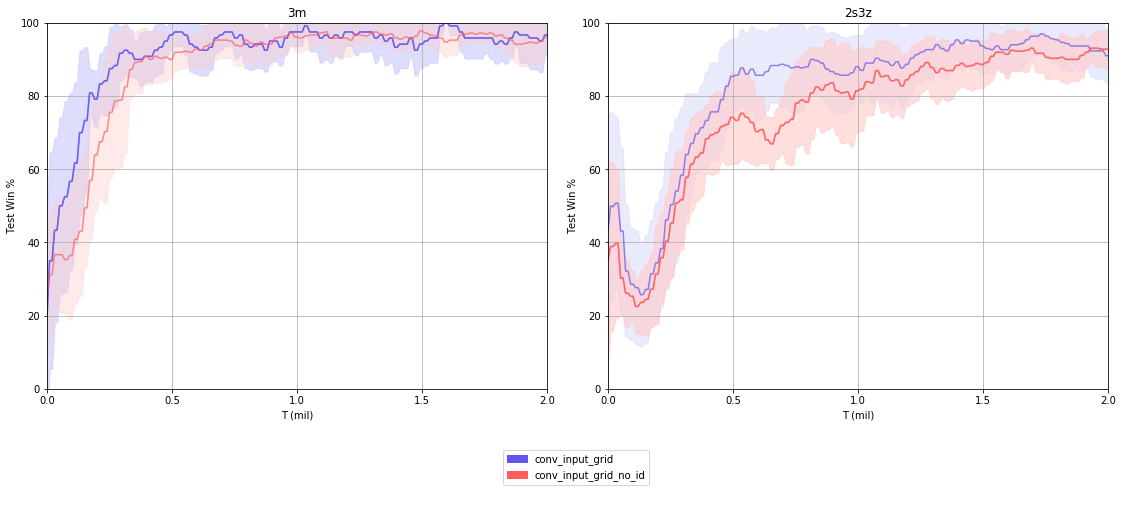
\includegraphics[scale=0.47]{images/graphs/noid.png}}
    \caption{Mean test win rates of the \textbf{conv\_input\_grid} and \textbf{conv\_input\_grid\_no\_id} architectures. The shaded region shows one standard deviation above and below the mean. There does not appear to be any significant decrease in performance without the ID observation, on either the 3m or 2s3z map.}
    \label{fig:noid}
\end{figure}


Clearly, the architecture suffered very little decrease in performance on both maps. Even though agents share network weights, these results suggest that the network can differentiate between the agents somehow (or that this differentiation is not necessary for good performance), thus rendering the agent ID unnecessary. 


\subsubsection{Agent Differentiation}

The network may be able to perform this differentiation through the use of its GRU-cell.

We can therefore make the following hypothesis:

\begin{hyp}[Agent Differentiation] \label{hyp:second}
In a non-recurrent network, two action-observation histories arising from two different agents may not be able to be locally disambiguated from the network's input, leading to reduced performance.
\end{hyp}


Hypothesis 2 is easily tested by removing the GRU-cell from the \textbf{conv\_input\_grid\_no\_id} architecture and performing the same experiment to measure performance; the network cannot disambiguate two different action-observation histories from two different agents without a recurrent unit, as the agents share network weights. The result of this experiment is shown in figure \ref{fig:RNNvsnonRNN}.

\begin{figure}
    \centering
    \hbox{\hspace{5em}\includegraphics[scale=0.5]{images/graphs/RNN.png}}
    \caption{Mean test win rates of the \textbf{conv\_input\_grid\_no\_id} with and without a GRU-cell before the final linear layer. The shaded region shows one standard deviation above and below the mean. There appears to be no significant decrease in performance.}
    \label{fig:RNNvsnonRNN}
\end{figure}


We can see that, despite a small decrease in performance, the network is still learning fairly effectively. A likely reason for  this result is that the environment is largely deterministic. This means that the architecture does not need to formulate extensive belief states, which is where RNNs are extremely useful \cite{beliefstate}. 

This result suggests that Hypothesis 2 is invalid, since the lack of agent disambiguation (in the non-recurrent network) does not appear to be a bottleneck for performance in these tasks.

\subsubsection{Network Inputs}

It is important for us to understand which observations are required for good performance. To do this, we run experiments in the same way as before on the \textbf{conv\_input\_grid\_no\_id} architecture. However, we vary the amount of information included in the observation, from very rich to empty (note that we always pass a particular available action as an input, so even with an empty observation the network does receive an input). This allows us to clearly see the effect of each observation on performance, as well as to see the base level of performance provided by the input actions.

The level of observations we will use are shown below. The row headers are the names of the observation levels (which are referred to in figure 16), and the column headers are observation features (a checkmark indicates that a particular feature is included in an observation level). Note that an available action is always included as an input to the network (although strictly is not an observation, but is included here for clarity).

\begin{adjustwidth}{-.5in}{-.5in}  
\begin{center}
\begin{tabular}{|l|l|l|l|l|l|} 
\hline
              & Agent ID & Unit Type & Health & Ally or Enemy Unit? & Available Action  \\ 
\hline
Full      &  \centering\checkmark    &    \checkmark   &          \checkmark          &    \checkmark                &       \checkmark \\ 
\hline
No ID    &    &  \centering\checkmark      &    \checkmark                   &         \checkmark              &     \checkmark      \\ 
\hline
No ID or Unit Type        &       &       & \centering\checkmark                    &     \checkmark                  &\checkmark           \\ 
\hline
Only Ally or Enemy &     &        &                   &       \centering\checkmark              &    \checkmark       \\
\hline
Empty &       &      &                   &                  &  \checkmark\\
\hline
\end{tabular}
\end{center}
\end{adjustwidth}

\vspace{5mm}
The relative performance of the architecture with these level of observations can be seen in figure \ref{fig:obs}. 

\begin{figure}
    \centering
    \hbox{\hspace{5em}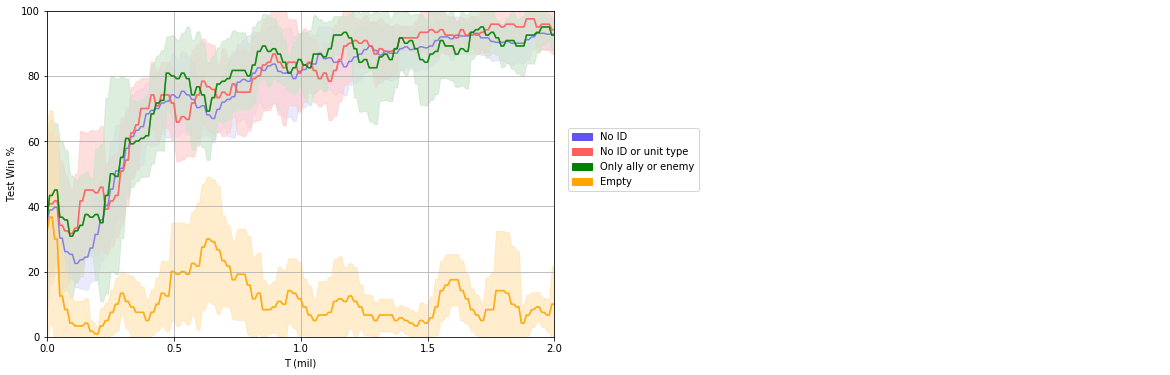
\includegraphics[scale=0.5]{images/graphs/obs.png}}
    \caption{Mean test win rate of the \textbf{conv\_input\_grid\_no\_id} with various levels of observation detail. The shaded region shows one standard deviation above and below the mean. The only required observation feature appears to be \textbf{ally\_or\_enemy} (which distinguishes between ally and enemy units).}
    \label{fig:obs}
\end{figure}

As expected, an empty observation gives very poor performance; the network cannot seem to learn at all. Surprisingly, however, every other level of observation showed near identical performance, reaching at least a $95\%$ win rate after just 2 million timesteps. This suggests that the only observation that is necessary for high performance in this architecture is \textbf{ally\_or\_enemy} (which distinguishes between ally and enemy units): an effective strategy of every agent shooting the same target can be performed using only this observation.










\subsection{Transfer and Multi-Task Learning}

Finally, with our task invariant architecture (\textbf{conv\_input\_grid\_no\_id}) we are able to start testing our partial observability hypothesis (Hypothesis 1) by evaluating the performance of the architecture in various transfer learning and multi-task learning situations.

To start, we will experiment upon transfer learning between the simple (single unit type) maps, 3m, 5m and 8m. We simply take a previously trained model for the relevant map, and begin training this network on another map. We will then compare the performance of this network (which has previously been trained on another map) with a network that was only trained on this map. Initially, we will only experiment with transfer learning between 3m and 5m, and 5m and 8m, to ensure the maps are as similar as possible, in line with our partial observability hypothesis.

Under the assumption of this hypothesis, we should see immediate benefit from having been trained on another map, because (under our hypothesis) the maps look similar due to the partial observability of the agents. Therefore, we expect a network that has been warm-started on another map to initially exhibit superior performance (hopefully close to the maximum win rate of the network on the map it was trained on) when compared to the standard network.


Firstly, we use a network that has reached the limit of performance for the warm-start of training on a different map. For 3m, 5m and 8m, this is after 600,000 timesteps.


We see in figure \ref{fig:transfer6} that this is not the case. In fact, we see the opposite result in some cases: warm-start training appears to be a disadvantage in some scenarios. In the 3m to 5m transfer case, we see that the network is unable to learn at all until around 200,000 timesteps, while a fresh network learns immediately.

\begin{figure}[h]
    \centering
    \hbox{\hspace{-5em}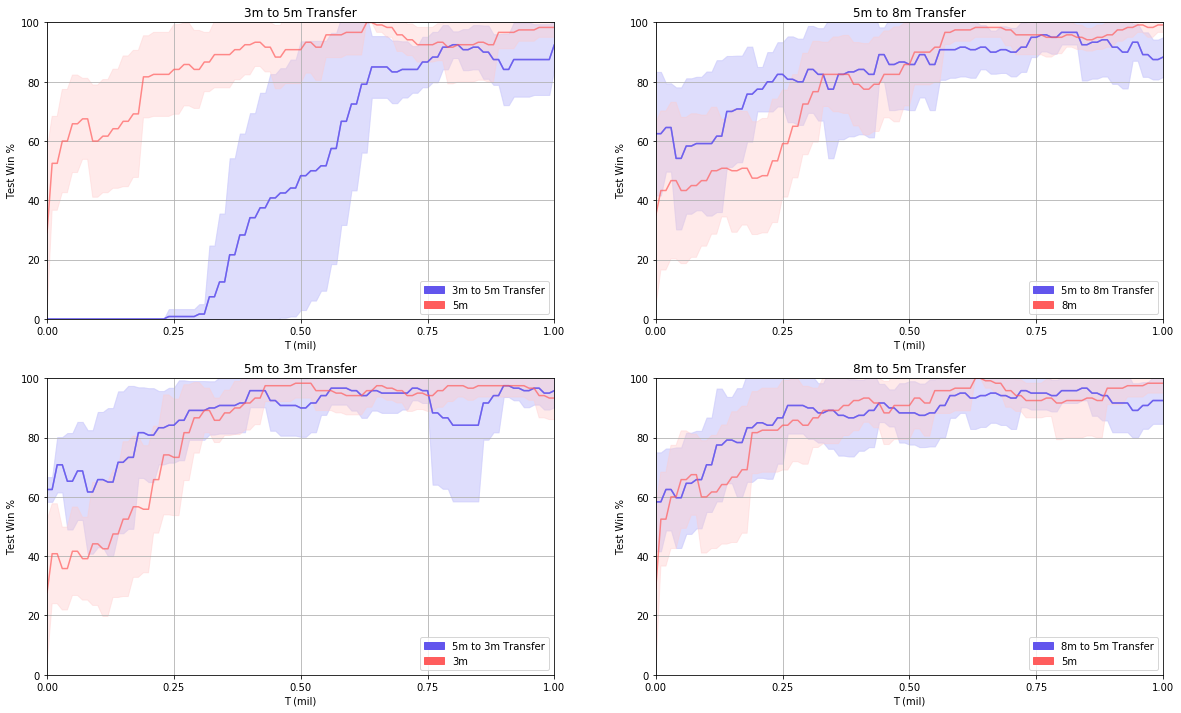
\includegraphics[width=1.2\textwidth]{images/graphs/6.png}}
    \caption{Mean test win rate of the \textbf{conv\_input\_grid\_no\_id} architecture on various scenarios using warm-start training (using a network that has trained already trained for 600,000 timesteps on another scenario). The shaded region shows one standard deviation above and below the mean. This format of transfer learning does not appear to be useful for training and, in some cases, it appears to have a negative effect. }
    \label{fig:transfer6}
\end{figure}


The reason for this may be that the network has over-fitted the original map, and is no longer ``plastic'' enough to learn on another map (the term ``plastic'' here refers to a network's ability to respond to training). The time where no progress is made in the 3m to 5m transfer example can thus be characterised as a period of ``undoing'' the previous work, in order to be able to learn on this new map.

To test this, we shall try again with networks that have not yet reached limit performance, but have shown some good progress, which is around 200,000 timesteps. At this point, the network is still very ``plastic'', and able to adapt to other maps, but still has learned a good insight into the game. This experiment is shown in figure \ref{fig:transfer2}.


\begin{figure}[h]
    \centering
    \hbox{\hspace{-5em}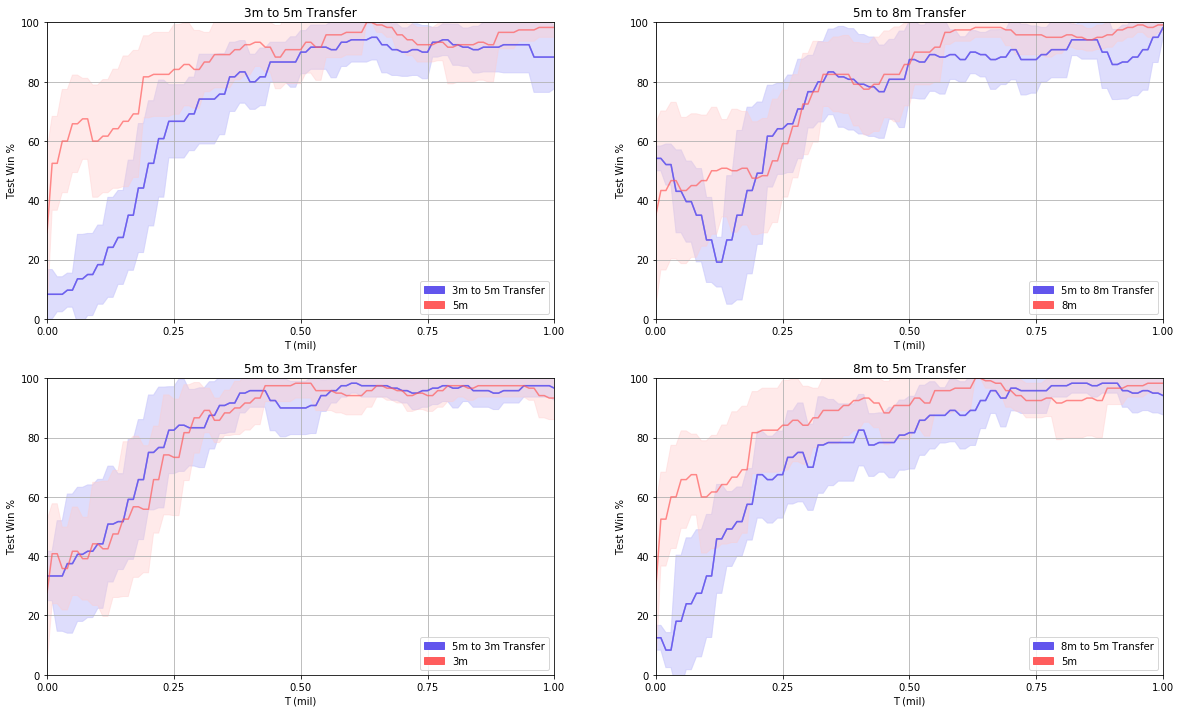
\includegraphics[width=1.2\textwidth]{images/graphs/2.png}}
    \caption{Mean test win rate of the \textbf{conv\_input\_grid\_no\_id} architecture on various scenarios using warm-start training (using a network that has trained already trained for 200,000 timesteps on another scenario). The transfer does not appear to aid with training, and in some cases can be seen to negatively impact it.}
    \label{fig:transfer2}
\end{figure}

We see a similar result: the warm-start of training does not provide any benefit. We do see an improvement in the 3m to 5m transfer case, as the network immediately starts to make progress, but it is still nowhere close to the high initial performance that we expected.

However, another observation that can be made is that transfers from larger maps to smaller maps are more successful than vice-versa. This is likely due to the fact that the agents in a larger map are trained on scenarios it will likely experience in a smaller map, but the converse is not necessarily true.


A likely explanation for these results is that the input space is simply too different for a different map. Although the environment is partially observable, agents in different maps will observe a different number or enemies and allies a large amount of the time, especially if the observation radius includes all other enemies (which is very likely during the later stages of the battle when the units are closer together). 

Hence, we devise a strategy for a network to learn on multiple maps simultaneously, to enrich the input space and allow for a more generalisable network. We maintain a network during training, and for each episode, we choose a map uniformly at random from a set of available maps, and train on that episode as normal. We will start with learning on just two maps, 3m and 5m.

The results of this multi-task learning experiment can be seen in the top left graph in figure \ref{fig:reptileall}. 




\begin{figure}[h]
    \centering
    \hbox{\hspace{-5em}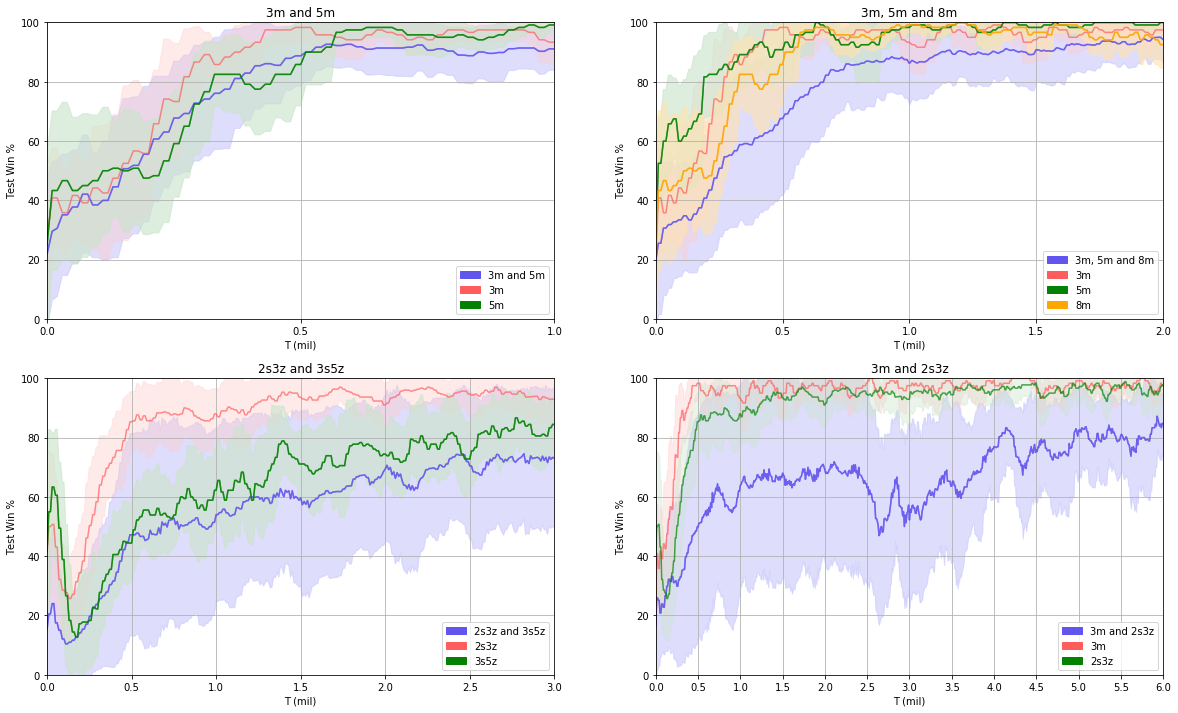
\includegraphics[width=1.2\textwidth]{images/graphs/all.png}}
    \caption{Mean test win rate of the \textbf{conv\_input\_grid\_no\_id} architecture training various sets of maps simultaneously. The shaded region shows one standard deviation above and below the mean. The network can be seen to reach high performance on multiple maps simultaneously.}
    \label{fig:reptileall}
\end{figure}


Excellent performance is exhibited on both maps, showing similar performance to when the architecture was trained on 3m and 5m individually.  

A natural extension to this experiment is to try to learn on more than 2 maps, or maps with more than one unit type. We therefore run two more experiments: one experiment on 3m, 5m and 8m, and one experiment on 2s3z and 3s5z. The results of these experiments are also shown in figure \ref{fig:reptileall}.



When trained on 3m, 5m and 8m, we can see only a small drop in performance and increase in variance when compared to the performance of training on the individual maps. A similar observation can be made when trained on 2s3z and 3s5z: the performance limit and final variance is close to those individual maps (although there is some decrease in performance), showing that, with enough training time, the network can achieve close to the highest performance possible on multiple maps.

When trained on both 3m and 2s3z, we do see a significant decrease in performance (increased convergence time and variance) when compared to the performance of training on the individual maps. This is likely because each map has an entirely different set of unit types, and therefore the maps are not very similar. However, the limit of performance is still high, suggesting the network can effectively learn both maps simultaneously.

Overall, under this new system of training on multiple maps simultaneously, we have shown that our task invariant architecture is able to learn across various tasks with some level of success, albeit with reduced performance in some cases. These results largely support our partial observability hypothesis (Hypothesis 1), but the decrease in performance suggests there are some differences between the tasks that cause difficulty for a single network.


\section{Alternative Approaches}
Machine learning is a vast field of computer science with many approaches available. Here we describe some of the alternate approaches that could have been taken.

\subsection{Transformer Networks}

Transformer networks are similar to RNNs in that they can be used to process sequenced data. However, they are able to process out-of-order sequences, which RNNs are unable to process effectively. Because of this, transformer networks are used extensively in natural language processing (NLP). This feature also allows for greater parrelization than RNNs.

A transformer network consists of a set of chained encoders and a set of chained decoders. Both the encoders and decoders make use of an attention mechanism: a mechanism to use a set of encodings to incorporate context into a sequence \cite{illustratedtransformer}. An attention function can be described as mapping a query and a set of key-value pairs to an output, where the query, keys, values, and output are all vectors. \cite{attention}. The output is computed as a weighted sum of the values, where the weight assigned to each value is computed by a compatibility function of the query with the corresponding key \cite{attention}.

Scaled dot-product attention is a specific attentuation function with the following definition, as described in \cite{attention}:

\[
Attention(Q,K,V)=softmax(\frac{QK^T}{\sqrt{d_k}})V
\]

Where $Q$, $K$, and $V$ are the matrices containing the queries, keys, and values respectively, with n being the dimension of the queries and keys.

Self-attention refers to the situation where the queries, keys, and values are all created using encodings of the sequence \cite{illustratedtransformer}.


Each encoder and decoder uses such an attention mechanism, which generates weights for each input when producing the output \cite{illustratedtransformer}.

Both the encoders and decoders have a feed-froward neural network for additional processing of the outputs \cite{illustratedtransformer}.

Although transformers have demonstrated great success in the field of NLP \cite{attention}, this architecture has also shown excellent results in other areas, including Starcraft II (AlphaStar used a transformer network in its architecture) \cite{alphastar}.

Therefore, this network architecture is a very promising approach in the Starcraft environment (and other similar environments) due to the network's superior ability to estimate the relevance of specific inputs in sequence data.


\subsection{Graph Convolutional Reinforcement Learning}

An alternative approach is to model the environment as a graph, as described in \cite{graph}. This builds on some of the ideas explored in this paper, but formalises the relationships between agents (and other units) using a graph. Each agent is represented by a node in the graph, and each node $i$ has a set of neighbours $\mathbb{B}_i$ which is determined by distance or other metrics \cite{graph}.

\cite{graph} describes in detail a network architecture for environments represented in this way, called graph  convolutional reinforcement learning, namely DGN. DGN consists of three types of modules:  observation encoder, convolutional layer and Q-network. For agent $i$ at time step $t$, the observation encoder encodes partial observtaion $o_i^t$ into latent feature $h_i^t$ \cite{graph}. The convolutional layer integrates the feature vectors in the local region (including node $i$ and its neighbors $\mathbb{B}_i$) and generates the latent feature vector $h′^t_i$. By stacking more convolutional layers, the receptive field of an agent gradually grows, where more information is gathered, and thus the scope of cooperation can also increase \cite{graph}. The final latent feature is then used as input into the Q-network as normal.

DGN shares weights among all agent, making it easy to scale, and has shown great success in various game examples \cite{graph}. Therefore, applying this technique to the Starcraft II environment has a lot of potential, especially considering the successes of convolutional neural networks in this project. 

A downfall of this approach is that it is not invariant to the number of agents, since the size of the graph is defined in terms of this. A possible way to adapt this is, perhaps, to make each node a specific location in the environment, and assign weights to the edges with respect to agent locations. For example, edge $e_i = (u,v)$ has finite weight if, and only if, there are two agents close to the locations represented by nodes $u$ and $v$ respectively.


\iffalse
\subsection{Actor-Critic Methods}


Counterfactual Multi-Agent Policy Gradients (COMA) is a multi-agent reinforcement learning algorithm that uses a centralised critic to estimate the Q-function
and decentralised actors to optimise the agents' policies \cite{coma}. The algorithm also uses a \textit{counterfactual baseline} that marginalizes out a single agent's action to address the challenges of agent credit assignment \cite{coma}. Each agent learns from a shaped reward $D^d=r(s,\textbf{a}) - r(s,(\textbf{a}^{-d},c^d$, where $d$ is the agent and $\textbf{a}$ is the joint action \cite{coma}. The global reward is compared to the reward received when the action of agent $d$ is replaced with a \textit{default action} $c^d$. The intuition behind this is that if an action improves $D^d$, then this action also improves the true global reward.

More details can be found in \cite{coma}.
\fi


\section{Conclusion}
\subsection{Summary of Results}

The main result from this report concerns training and testing on multiple scenarios using our task-invariant architecture. We found that transferring to an unseen scenario exhibited very poor performance (although performance was less poor when transferring to a smaller map). This is likely because of the ``out-of-distribution'' \cite{ood} problem: faced with a sample outside the training distribution, as neural network will generalise arbitrarily badly. This is particularly relevant to RNNs, where one observation difference in the entire history can lead to completely different hidden states. This also supports why we saw a slight improvement when transferring from larger to smaller maps: if the network has seen similar states, the transfer is more successful.



However, we found that multi-task learning was more successful, suggesting that this ``out-of-distribution'' problem is resolved through this style of learning. Furthermore, this indicates that a single network has a far greater capacity for learning than a single scenario. Moreover, this shows that the various tasks are in fact closely linked: we have shown that these scenarios can be played somewhat well by a generalisable architecture trained over each map, which supports our partial observability hypothesis \cs{state what that hypothesis is, or reference where it is defined}.



Finally, we found that the memory requirements for architectures utilising grid-based observations and actions to be extremely large (~5Gb per network, compared to under 1Gb for non-grid-based architectures for small maps). This is a major downfall of the approach, as it limits the size the map that can be trained upon, and increases the training time \cs{Ok, but surely you could use a smaller replay buffer or even on-policy methos or otherwise mitigate the problem, or just lower grid resolution?}.





\subsection{Future Work}

Due to the size and scope of this project there are a number of directions in which it can be continued or improved. We detail some of the most promising avenues here.


\subsubsection{Task Invariance Using QMIX}

The QMIX mixing network is inherently dependent on the task: the number of inputs in the network depends on the number of agents. The VDN mixing network does not have this problem, it simply sums the $Q$-values of each agent. Future work could involve adapting the QMIX mixing network for task invariance. This would involve a transformer-style architecture to process a new representation of the state that is independent of the number of units in the map.


\subsubsection{Observing Terrain}

The terrain of a StarCraft II map (high ground and low ground) can be particularly important information to aid with micromanagement. For example, attacking from high ground allows units to not be seen by the enemy (until the enemy is attacked), so it is an advantageous position to be in.

Currently, the agent architecture does not use this observation\cs{it's not really due to the architecture, we just don't feed in the features}, but it would be useful to evaluate its effectiveness.


\subsection{Personal Development}
This project allowed me to explore my passion for Reinforcement Learning. In particular, I was able to implement and appreciate various concepts from the Machine Learning course, such as convolutional neural networks, as well as evaluating them using state-of-the-art hardware.

Furthermore, the scope of this project was larger than anything previously undertaken, which gave me an invaluable insight into collaborative research by using open-communication channels, version control of a large shared repository, as well as discussions with various other lab members. This project has also been used by the lab to work towards a more general multi-agent RL algorithm.

\bibliographystyle{plain}
\bibliography{bib}
\end{document}
